% !TEX program = xelatex
% ============================================================
%  全国大学生数学建模竞赛 (CUMCM) LaTeX 通用论文模板
%  编译方式: XeLaTeX
% ============================================================
\documentclass[12pt,a4paper]{ctexart}

% ======================== 宏包加载 ========================
\usepackage[top=2.5cm, bottom=2.5cm, left=2.8cm, right=2.8cm]{geometry}
\usepackage{amsmath, amssymb, amsthm}
\usepackage{graphicx}
\usepackage{float}
\usepackage{subcaption}
\usepackage{booktabs}
\usepackage{array}
\usepackage{multirow}
\usepackage{longtable}
\usepackage{xcolor}
\usepackage{hyperref}
\hypersetup{
    colorlinks=true,
    linkcolor=blue!70!black,
    citecolor=green!50!black,
    urlcolor=blue!60!black
}
\usepackage{listings}
\lstset{
    basicstyle=\small\ttfamily,
    breaklines=true,
    frame=single,
    numbers=left,
    numberstyle=\tiny\color{gray},
    keywordstyle=\color{blue},
    commentstyle=\color{green!60!black},
    stringstyle=\color{red!70!black},
    tabsize=4
}

\usepackage{setspace}
\usepackage{indentfirst} % 使章节、小节标题后的首段也按正文规则缩进
\onehalfspacing
\setlength{\parindent}{2em} % 正文各段首行统一缩进两个汉字
\usepackage{enumitem}
\setlist{nosep, leftmargin=2em}
\usepackage{titlesec}
\usepackage{caption}
\captionsetup{font=bf, labelfont=bf}
\usepackage{bm}
\usepackage{mathtools}

% ======================== 字体设置 ========================
\setCJKmainfont{SimSun}[BoldFont=SimHei, ItalicFont=KaiTi]
\setCJKsansfont{SimHei}
\setCJKmonofont{FangSong}
\setmainfont{Times New Roman}
% 显式把 ctex 的 \songti/\heiti/\kaishu/\fangsong 族都配上粗体，避免
% 在摘要等使用 \songti 的环境里 \textbf{中文} 无法加粗（显示不出黑体）。
\setCJKfamilyfont{zhsong}{SimSun}[BoldFont=SimHei]
\setCJKfamilyfont{zhhei}{SimHei}[BoldFont=SimHei]
\setCJKfamilyfont{zhkai}{KaiTi}[BoldFont=SimHei]
\setCJKfamilyfont{zhfang}{FangSong}[BoldFont=SimHei]

% ======================== 编号格式 ========================
\renewcommand{\thesection}{\chinese{section}、}
\renewcommand{\thesubsection}{\arabic{section}.\arabic{subsection}}
\renewcommand{\thesubsubsection}{\arabic{section}.\arabic{subsection}.\arabic{subsubsection}}

% ======================== 标题格式 ========================
\titleformat{\section}
  {\centering\heiti\zihao{-3}\bfseries}
  {\thesection}{0em}{}
\titlespacing*{\section}{0pt}{1.5ex plus .5ex minus .2ex}{1.0ex plus .2ex}

\titleformat{\subsection}
  {\heiti\zihao{4}\bfseries}
  {\thesubsection}{1em}{}
\titlespacing*{\subsection}{0pt}{1.2ex plus .4ex minus .2ex}{0.8ex plus .2ex}

\titleformat{\subsubsection}
  {\heiti\zihao{-4}\bfseries}
  {\thesubsubsection}{1em}{}
\titlespacing*{\subsubsection}{0pt}{1.0ex plus .3ex minus .1ex}{0.6ex plus .1ex}

% ======================== 定理环境 ========================
\theoremstyle{definition}
\newtheorem{definition}{定义}[section]
\newtheorem{assumption}{假设}[section]
\theoremstyle{plain}
\newtheorem{theorem}{定理}[section]
\newtheorem{lemma}{引理}[section]
\newtheorem{proposition}{命题}[section]
\newtheorem{corollary}{推论}[section]
\theoremstyle{remark}
\newtheorem{remark}{注}[section]

% ======================== 自定义命令 ========================
\renewenvironment{abstract}
  {{\centering\heiti\zihao{-3}摘\quad 要\par}\vspace{0.5em}\zihao{-4}\songti}
  {\par\vspace{1em}}

\newcommand{\keywords}[1]{%
  \par\noindent\textbf{关键词：}#1}

\newcommand{\upcite}[1]{\textsuperscript{\cite{#1}}}

\newenvironment{symboltable}
  {\begin{center}\zihao{5}\begin{tabular}{>{\centering\arraybackslash}p{3.5cm} p{7.5cm} >{\centering\arraybackslash}p{1.5cm}}
  \toprule
  \textbf{符号} & \textbf{含义} & \textbf{单位} \\
  \midrule}
  {\bottomrule\end{tabular}\end{center}}

\newcommand{\step}[1]{\par\noindent\textbf{Step #1}\quad}

% ============================================================
\begin{document}
\pagestyle{plain}
\setcounter{page}{1}
\pagenumbering{arabic}
\begin{center}
{\zihao{-2}\heiti\bfseries Ward 层次聚类与符号约束 STIRPAT-岭回归下的碳排放分类与预测}
\end{center}

\begin{abstract}
我国已明确提出2030年前碳达峰与2060年前碳中和目标。研究碳排放的时空特征、关键驱动因素、发展趋势与治理对策，对推进绿色转型具有重要意义。本文根据碳排放数据及国家统计年鉴中的能源结构资料，采用\textbf{全局Moran检验、Ward层次聚类、带符号约束STIRPAT-ridge回归、多情景路径递推和政策规则测算}等方法，对省份进行分类，识别碳排放驱动因素，分析2026至2045年碳排放总量与强度并判断碳达峰，最后编制分区域、分部门、分阶段的政策建议书。

\textbf{针对问题一，}本文建立排放规模、人均排放、排放强度、煤炭排放占比与过程排放占比五维指标体系，通过\textbf{全局Moran检验}判断省域空间差异，并利用\textbf{Ward层次聚类}进行省份分类。结果表明，30省可分为高规模高压力型、低规模相对低碳型和北京结构差异簇三类。

\textbf{针对问题二，}本文建立\textbf{带符号约束STIRPAT-ridge回归模型}识别驱动因素，并利用留一交叉验证选择岭参数、利用扩展窗口回测检验外推表现。结果表明，\textbf{GDP}呈正向作用，\textbf{清洁能源比重}呈负向作用；该结构模型用于解释驱动方向并为情景推演提供输入接口。

\textbf{针对问题三，}本文采用\textbf{多情景路径递推方法}，比较基准、低碳与强化低碳情景下的碳排放总量和强度。结果表明，三情景总量均平缓上升，始终满足强化低碳低于低碳低于基准，强度均持续下降，\textbf{预测期内未见碳达峰}。

\textbf{针对问题四，}本文依据前三问结论建立\textbf{省级政策规则与阶段监测指标体系}，从区域、部门和阶段三个层面编制政策建议书。建议对高规模高压力型省份加强总量控制、煤炭替代与能效改造，优先推进工业和电力部门减排，并按三个阶段开展滚动监测。
\end{abstract}

\keywords{碳排放分析、空间自相关、聚类分类、STIRPAT-ridge、情景预测}

\section{问题重述}

\subsection{问题背景}
二氧化碳（CO₂）是温室气体排放的主要构成成分。其过度排放会加剧温室效应、扰乱气候系统、破坏生态环境，并对全球可持续发展构成严峻挑战。改革开放以来，我国经济高速增长的同时能源消费总量不断攀升，目前碳排放规模居全球前列。同时，我国高度重视碳减排工作，我国提出碳达峰、碳中和目标，启动全国碳排放权交易市场，并持续强调要积极稳妥推进碳达峰碳中和工作。

因此，准确把握碳排放的时空演变特征、识别关键驱动因素、科学研判未来趋势并提出切实可行的应对策略，是实现“双碳”战略目标的重要基础。这不仅有助于持续改善我国生态环境质量，也有利于应对全球气候变化带来的压力，促进经济社会绿色转型，最终推动形成人与自然和谐共生的现代化格局。

\subsection{问题提出}

\textbf{问题 1：}根据附件1和附件2中的碳排放数据，分析我国各省份在碳排放核心指标上是否存在显著的空间差异；并围绕碳排放规模、排放效率及其与经济发展的关联程度，构建多维度的分类分级评价指标体系，进而对各省份进行类型划分与等级判定。

\textbf{问题 2：}结合中国统计年鉴中能源结构等相关数据，探究影响碳排放变化的基本因素，并据此建立碳排放预测模型。

\textbf{问题 3：}以问题2中所确定的最优预测模型为基础，分别设定基准情景、低碳情景和强化低碳情景三种发展场景，预测2026—2045年我国碳排放总量及碳排放强度的变化趋势，并判断碳达峰可能出现的时间节点与峰值水平。

\textbf{问题 4：}综合上述分析结果以及我国碳达峰、碳中和的战略目标，撰写相应的政策建议书。

\section{问题分析}

\subsection{问题一的分析}
问题一要求判断各省碳排放核心指标是否存在显著空间差异，并围绕规模、效率与经济关联度建立指标体系完成分类，属于2022年30个省级地区的横截面识别问题。本文按指标建立、空间检验、聚类分类与重点治理识别的路线展开。

指标建立方面，排放规模用于反映总量，人均排放与排放强度用于反映人口和经济效率，煤炭排放占比与过程排放占比用于反映能源和产业结构。由于缺少跨省贸易流、能源流等直接经济联系数据，后三项仅作为经济关联的结构代理。考虑到五项指标量纲不同，本文先进行标准化。空间检验方面，本文建立省域邻接权重矩阵，采用全局Moran检验\upcite{moran}与置换检验判断空间集聚，并对无陆上邻居的海南设置桥接关系。聚类分类方面，本文采用Ward层次聚类\upcite{ward}，并在$k=2,\ldots,6$中用轮廓系数选择类别数。候选范围兼顾30个样本的类别规模，避免产生过多小簇。重点治理识别采用前20\%规则，以便在有限治理资源下保留约五分之一的优先对象；10\%对应省份过少，25\%则会削弱重点性。若轮廓系数整体偏低，分类只作为省份画像，不解释为稳定的行政边界。

\subsection{问题二的分析}
问题二要求结合中国统计年鉴中的能源结构数据\upcite{stats}识别影响碳排放的基本因素，并建立碳排放预测模型。考虑到附件1聚合为全国年度序列后仅有2019--2024年6个有效样本，属于小样本年度驱动分析问题，本文拟按因素识别与预测建模两步展开，其核心是构建带符号约束的STIRPAT-ridge回归模型。

因素识别方面，人口、GDP、煤炭占比与清洁能源比重存在共线性，直接回归容易出现系数不稳。本文基于STIRPAT框架建立对数线性方程，引入岭惩罚并施加方向约束。人口与煤炭占比的系数可能落在零边界，因此只解释被模型保留的方向，不把贴界变量写成已被稳定识别。参数选择采用留一交叉验证，外推表现采用扩展窗口并与时间趋势基线比较。结构模型的外推误差可能高于简单基线，因此模型取舍同时考虑方向解释、情景变量接口和回测误差，不以单一MAE宣称最优。2025年数据按历史同期占比年化，其数值与计算过程放在数据预处理部分。

\subsection{问题三的分析}
问题三要求利用问题二的结构模型设置三种情景，分析2026--2045年碳排放总量与强度并判断达峰情况。本问不重新估计系数，而是采用多情景路径递推方法比较不同外生路径。该方法不含排放对GDP和能源结构的内生反馈，因此属于条件情景测算，而非系统动力学演化模型。

三种情景由GDP、人口和能源结构路径共同决定，达峰判断对GDP增速与能源调整步长较为敏感。正文将公开各阶段GDP增速和能源步长，并说明人口增速、占比边界及校准系数的用途。三情景使用同一校准系数，只调整共同尺度，不改变情景间的相对排序。若最大值落在2045年窗口右端，只能说明预测期内未达峰，不能据此认定2045年已经达峰或给出最终峰值。

\subsection{问题四的分析}
问题四要求把前三问结论转化为政策建议。本文建立由省级规则、类别覆盖率、部门排序与阶段指标组成的可计算规则体系，而不把示性函数和份额汇总称为政策仿真模型。

总量控制采用前20\%阈值，是为了筛出少量优先治理省份；能效、煤炭替代、市场机制和需求侧治理采用中位数阈值，是为了进行覆盖面更广的工具筛选。随后按问题一类别汇总规则触发率，按部门累计排放份额确定治理顺序，并根据问题三的排放强度建立阶段监测指标。这些规则用于组织建议对象与监测顺序，不计算政策实施后的实际减排量。


\section{模型假设}

\begin{enumerate}[label=(\arabic*)]
\item 附件1中\texttt{Total}等于国内航空、地面交通、工业、电力和居民五部门之和，国际航空单列不计入。
\item 2025年数据仅覆盖前三季度，其年化值仅作模型衔接锚点，不视为完整年度统计。
\item 仅考虑人口、GDP、煤炭占比与清洁能源比重等核心驱动因素，忽略技术进步等次要因素的影响。
\item 不考虑重大突发事件、极端灾害与能源供应中断等小概率事件的冲击。
\item 省界相邻近似刻画省级空间联系，海南以广东、广西桥接，空间检验仅作探索性识别。
\item 人口、GDP与煤炭占比系数非负，清洁能源比重系数非正，该约束表达建模先验而非因果。
\item 2026至2045年外生路径仅代表本文设定的情景，不代表官方规划，亦非严格置信区间。
\end{enumerate}

\section{符号说明}
主要符号见表\ref{tab:symbol}。省级强度与全国预测强度使用的GDP单位不同，本文在对应章节中分别标注，避免将$\mathrm{t}/(\text{万元 GDP})$与$\mathrm{Mt}/(\text{万亿元 GDP})$混用。

\begin{table}[H]
\centering
\caption{主要符号及含义}
\label{tab:symbol}
\zihao{5}
\begin{tabular}{>{\centering\arraybackslash}p{2.7cm}>{\raggedright\arraybackslash}p{7.2cm}>{\centering\arraybackslash}p{2.0cm}}
\toprule
符号 & 含义 & 单位\\
\midrule
$C_t$ & 第$t$年全国二氧化碳排放量 & Mt CO$_2$\\
$E_i$ & 第$i$个省份排放规模 & Mt CO$_2$\\
$PC_i$ & 第$i$个省份人均排放 & t/person\\
$EI_i$ & 第$i$个省份单位GDP排放强度 & t/(万元 GDP)\\
$S_t^{coal}$、$S_t^{clean}$ & 全国煤炭比重、清洁能源比重 & $[0,1]$\\
$P_t$、$G_t$ & 全国人口、GDP & 万人、万亿元\\
$w_{ij}$ & 省份$i$与$j$之间的空间权重 & 无量纲\\
$\lambda$ & 岭回归正则化参数 & 无量纲\\
$I_t^{GDP}$ & 全国排放强度$C_t/G_t$ & Mt/(万亿元 GDP)\\
\bottomrule
\end{tabular}
\end{table}

\section{数据预处理}

为消除多源异构数据在时间尺度、统计口径和量纲上的差异，保证后续空间检验、宏观回归与情景推演的顺利进行，本文进行了四步数据预处理：

\paragraph{\textbf{步骤一：全国日频数据清洗与部门加总核验。}}
读取附件1提供的2019年1月1日至2025年9月30日全国日频碳排放数据集（包含\texttt{Total}总量与国内六大部门记录，共2465个观测日）。对逐日记录进行口径守恒核验，遍历检验全国总量\texttt{Total}与国内五大主要部门（电力、工业、地面交通、居民消费、国内航空）排放量之和的一致性。核验表明，逐日最大绝对误差仅为$2.0\times10^{-6}\ \mathrm{Mt}$，属于浮点计算微小截断误差，验证了数据源在部门加总层面的严格自洽性。核验后按年份将日频数据汇总为年度时间序列（保留2019--2024完整年度用于宏观驱动回归估计）。

\paragraph{\textbf{步骤二：2025年非完整年度排放量的季节性年化锚定。}}
由于附件1中2025年数据仅覆盖前三季度（1--9月），若直接与完整年度混合建模将引入系统性统计截断偏差。本文利用历史同期的季节平稳特征计算年化锚点。设$f_y$为历史年份$y$前三季度累计排放占全年总排放的比例，则2025年年化碳排放锚点$\widehat C_{2025}$定义为：
\begin{equation}
f_y=\frac{C_{y,1\text{--}9}}{C_{y,1\text{--}12}},\qquad
\widehat C_{2025}=\frac{C_{2025,1\text{--}9}}{\frac{1}{6}\sum_{y=2019}^{2024}f_y}=11639.658\ \mathrm{Mt\ CO_2}.
\label{eq:annualize}
\end{equation}
统计表明，2019--2024年历史同期比例均值$\bar f=0.740197$、样本标准差仅为$0.011311$（变异系数$1.53\%$），季节分布高度平稳。该年化值$\widehat C_{2025}=11639.658\ \mathrm{Mt}$仅作为连接问题二模型与问题三情景预测的连续性基准锚点，不参与历史回归训练，严格防范数据穿越。

\paragraph{\textbf{步骤三：省级排放清单与社会经济指标融合匹配。}}
读取附件2中30个省份的2022年排放清单（西藏自治区数据缺失予以客观剔除，有效样本容量$n=30$），提取各省范围一排放总量\texttt{Scope\_1\_Total}、煤炭排放量及工业过程排放量。将各省清单与国家统计局年鉴中的常住人口（万人）与地区生产总值（GDP，亿元）逐一对应起来，并对省名、样本量及指标完整性执行断言检验，确保数据无缺失与异常。

\paragraph{\textbf{步骤四：核心指标构建与多维特征无量纲化。}}
为消除人口与经济规模量纲差异，分别构建人均碳排放$PC_i$（$\mathrm{t/\text{人}}$）与单位GDP碳排放强度$EI_i$（$\mathrm{t/\text{万元 GDP}}$）：
\begin{equation}
PC_i=\frac{100E_i}{Pop_i},\qquad EI_i=\frac{100E_i}{GDP_i}.
\label{eq:q1-indicator}
\end{equation}
针对由排放规模$E_i$、人均排放$PC_i$、排放强度$EI_i$、煤炭排放占比$S_i^{coal}$与过程排放占比$S_i^{proc}$构成的五维特征空间，为消除不同指标绝对量纲与离散尺度差异（如规模指标跨越两个数量级），在进入降维与聚类前对特征实施对数压缩与$Z$-score标准化处理：
\begin{equation}
u_{ij}=\ln(1+x_{ij}),\qquad z_{ij}=\frac{u_{ij}-\mu_j}{\sigma_j},
\label{eq:q1-standard}
\end{equation}
其中$x_{ij}$为省份$i$在特征$j$上的原始观测值，$\mu_j$与$\sigma_j$分别为该特征在30省样本中的均值与标准差。变换后各指标方差齐性且初始权重均等，为后续Ward层次聚类提供了客观无偏的高维几何空间。

\section{模型建立与求解}

\subsection{问题一模型建立及求解}

\begin{figure}[H]
\centering

\includegraphics[width=0.90\textwidth]{figures/-问题一.drawio.png}
\caption{问题一流程图}
\label{fig:q1-flowchart}
\end{figure}

\subsubsection{模型建立}
\paragraph{模型来源与建模思路}
问题一同时考察省级排放的规模、效率、空间关联与结构差异。空间相关性采用经典的全局Moran's $I$统计量并利用蒙特卡洛置换检验评估显著性；省份分类采用基于式\eqref{eq:q1-standard}五维对数标准化特征的Ward层次聚类法。

空间权重矩阵遵循“共享省界即相邻”的地理邻接规则。记$w_{ij}$为省份$i$与$j$的空间权重，则
\begin{equation}
w_{ij}=\begin{cases}
1,& i\text{与}j\text{共享省界，或为海南与广东、广西的桥接关系},\\
0,& \text{其他情形},
\end{cases}\qquad w_{ii}=0.
\label{eq:q1-weight}
\end{equation}

该权重以省份是否共享省界为依据，用于检验地理邻近省份之间是否存在空间统计相关性。

Ward层次聚类以合并后组内离差平方和增量最小为准则。设类$A$与类$B$包含的省份数分别为$n_A,n_B$，中心向量分别为$\bar{\bm z}_A,\bar{\bm z}_B$，则两类合并的距离代价定义为：
\begin{equation}
\Delta(A,B)=\frac{n_A n_B}{n_A+n_B}\left\|\bar{\bm z}_A-\bar{\bm z}_B\right\|_2^2.
\label{eq:q1-ward}
\end{equation}
聚类始终在完整的五维标准化矩阵$\bm Z=(z_{ij})$上实施，PCA仅用于低维可视化展示。

\subsubsection{模型求解}
按式\eqref{eq:q1-indicator}计算30个省份的人均排放和排放强度，结合煤炭排放占比、过程排放占比构成五项指标。对任一指标$x_i$，依据式\eqref{eq:q1-weight}计算全局Moran's $I$：
\begin{equation}
I=\frac{n}{S_0}\frac{\sum_{i=1}^{n}\sum_{j=1}^{n}w_{ij}(x_i-\bar{x})(x_j-\bar{x})}{\sum_{i=1}^{n}(x_i-\bar{x})^2},\qquad S_0=\sum_{i=1}^{n}\sum_{j=1}^{n}w_{ij}.
\label{eq:moran}
\end{equation}
这里$n=30$，$\bar{x}$为省级指标均值，$I>0$表示相邻省份取值相似，$I<0$表示取值相异。在此基础上，固定随机种子对每一项指标随机置换999次，得到第$b$次置换的统计量$I^{(b)}$，以双侧经验$p$值衡量观测值$I^{obs}$的显著性：
\begin{equation}
p=\frac{1+\sum_{b=1}^{999}\mathbb{I}\left\{\left|I^{(b)}\right|\geq\left|I^{obs}\right|\right\}}{1000}.
\label{eq:q1-permutation}
\end{equation}
当$p<0.05$时，判定该指标在既定邻接权重下具有显著空间集聚；否则只保留描述性比较。在得到显著性结论的基础上，依据式\eqref{eq:q1-ward}的Ward合并准则自底向上逐步聚类，对候选类别数$k=2,\ldots,6$，由平均轮廓系数确定最优分类数：
\begin{equation}
S(k)=\frac{1}{n}\sum_{i=1}^{n}\frac{b_i-a_i}{\max\{a_i,b_i\}},\qquad k^*=\arg\max_{k\in\{2,\ldots,6\}}S(k),
\label{eq:q1-silhouette}
\end{equation}
其中$a_i$为省份$i$与同类样本的平均距离，$b_i$为其与最近异类样本的平均距离。最后以总量或强度处于样本前20\%作为重点治理的双入口规则：
\begin{equation}
P_i=\mathbb{I}\left\{E_i\geq Q_{0.8}(E)\ \text{或}\ EI_i\geq Q_{0.8}(EI)\right\}.
\label{eq:priority}
\end{equation}
$P_i=1$表示该省进入重点治理清单。

\subsubsection{结果展示}
\begin{figure}[H]
\centering
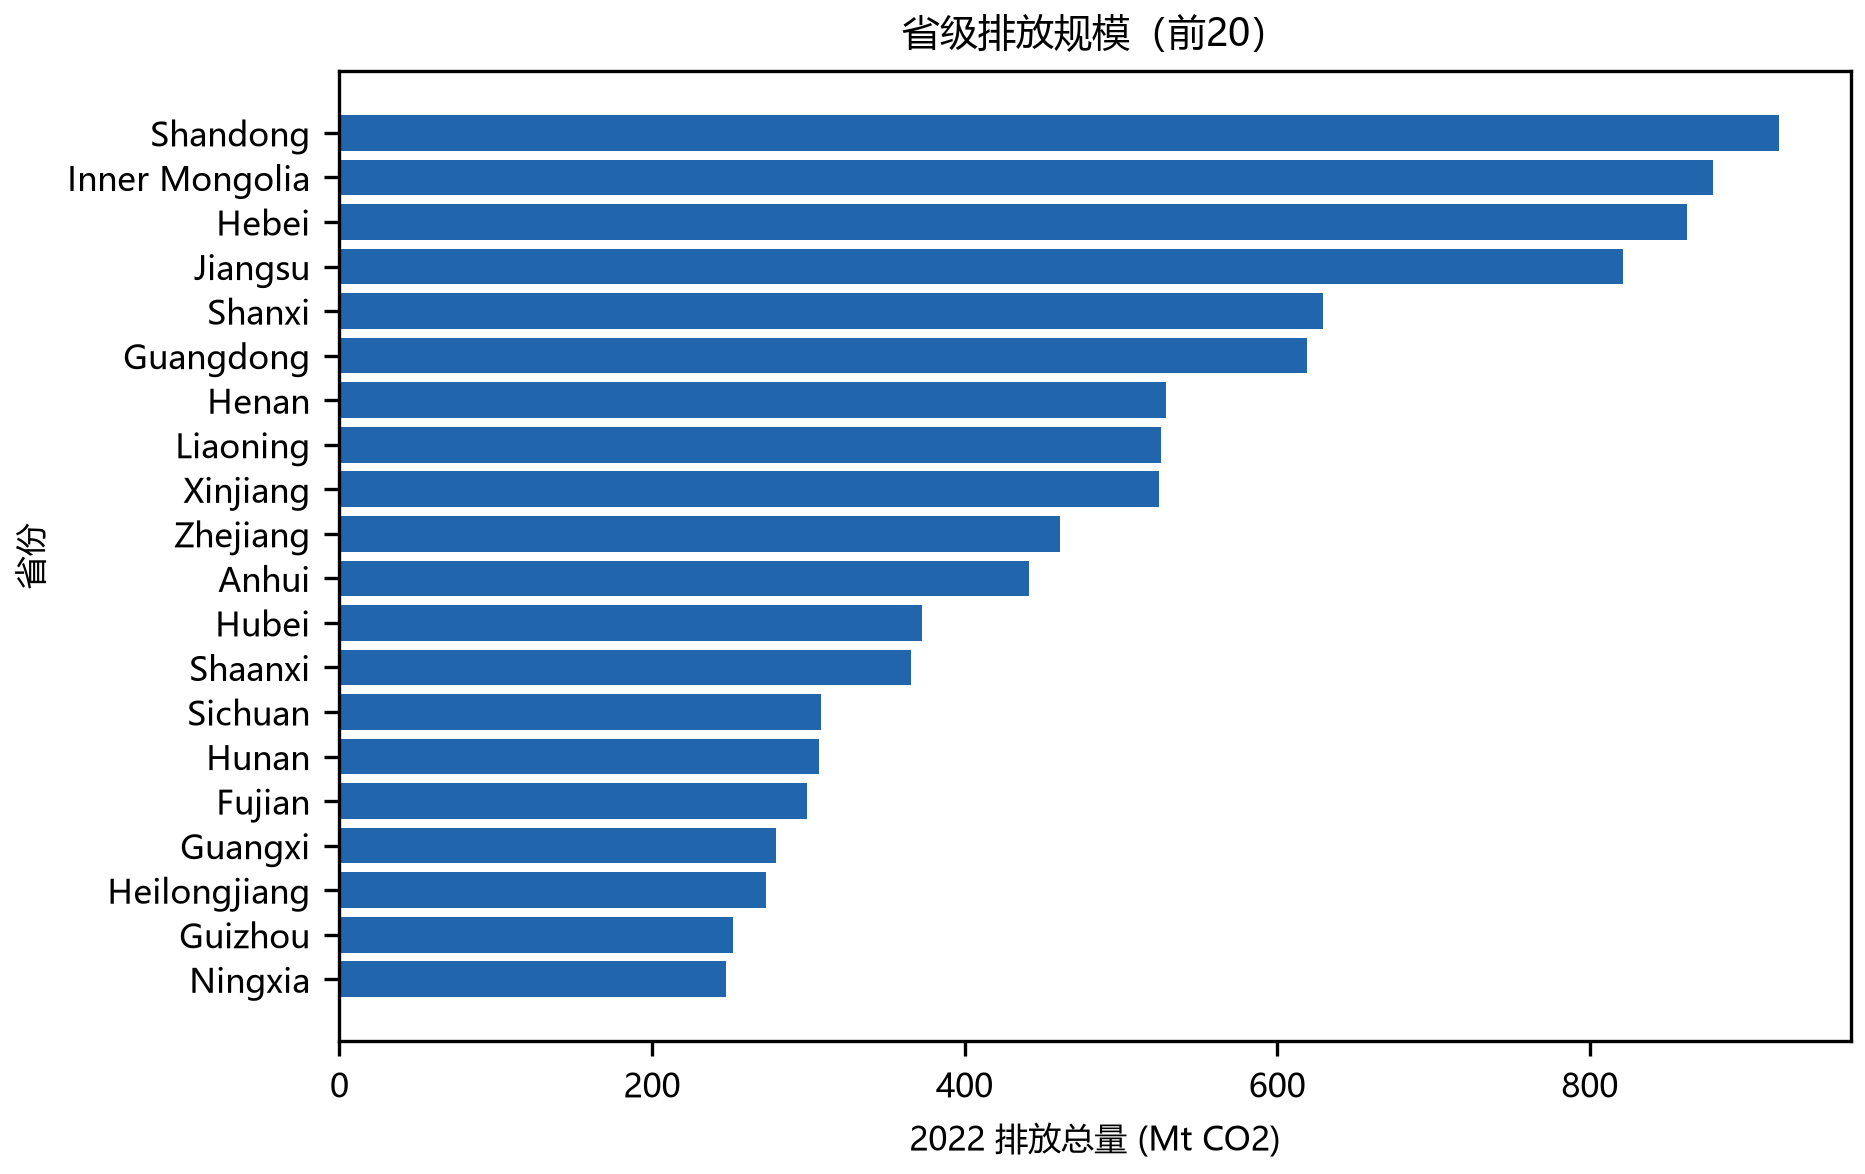
\includegraphics[width=0.7\textwidth]{figures/raw_q1_province_scale.png}
\caption{2022年省级排放规模前20省份（单位：Mt）}
\label{fig:q1-raw}
\end{figure}
\vspace{-0.4\baselineskip}
\nopagebreak[4]
图\ref{fig:q1-raw}显示，2022年省级排放规模呈现明显的头部集中格局，山东、内蒙古、河北等能源和工业大省位居前列，前20个省份即覆盖了样本排放的主体部分。排放总量与省份经济体量及能源消费结构高度相关，但仅凭总量排序无法反映排放效率差异，仍需结合强度与结构指标进一步识别。

\begin{figure}[H]
\centering
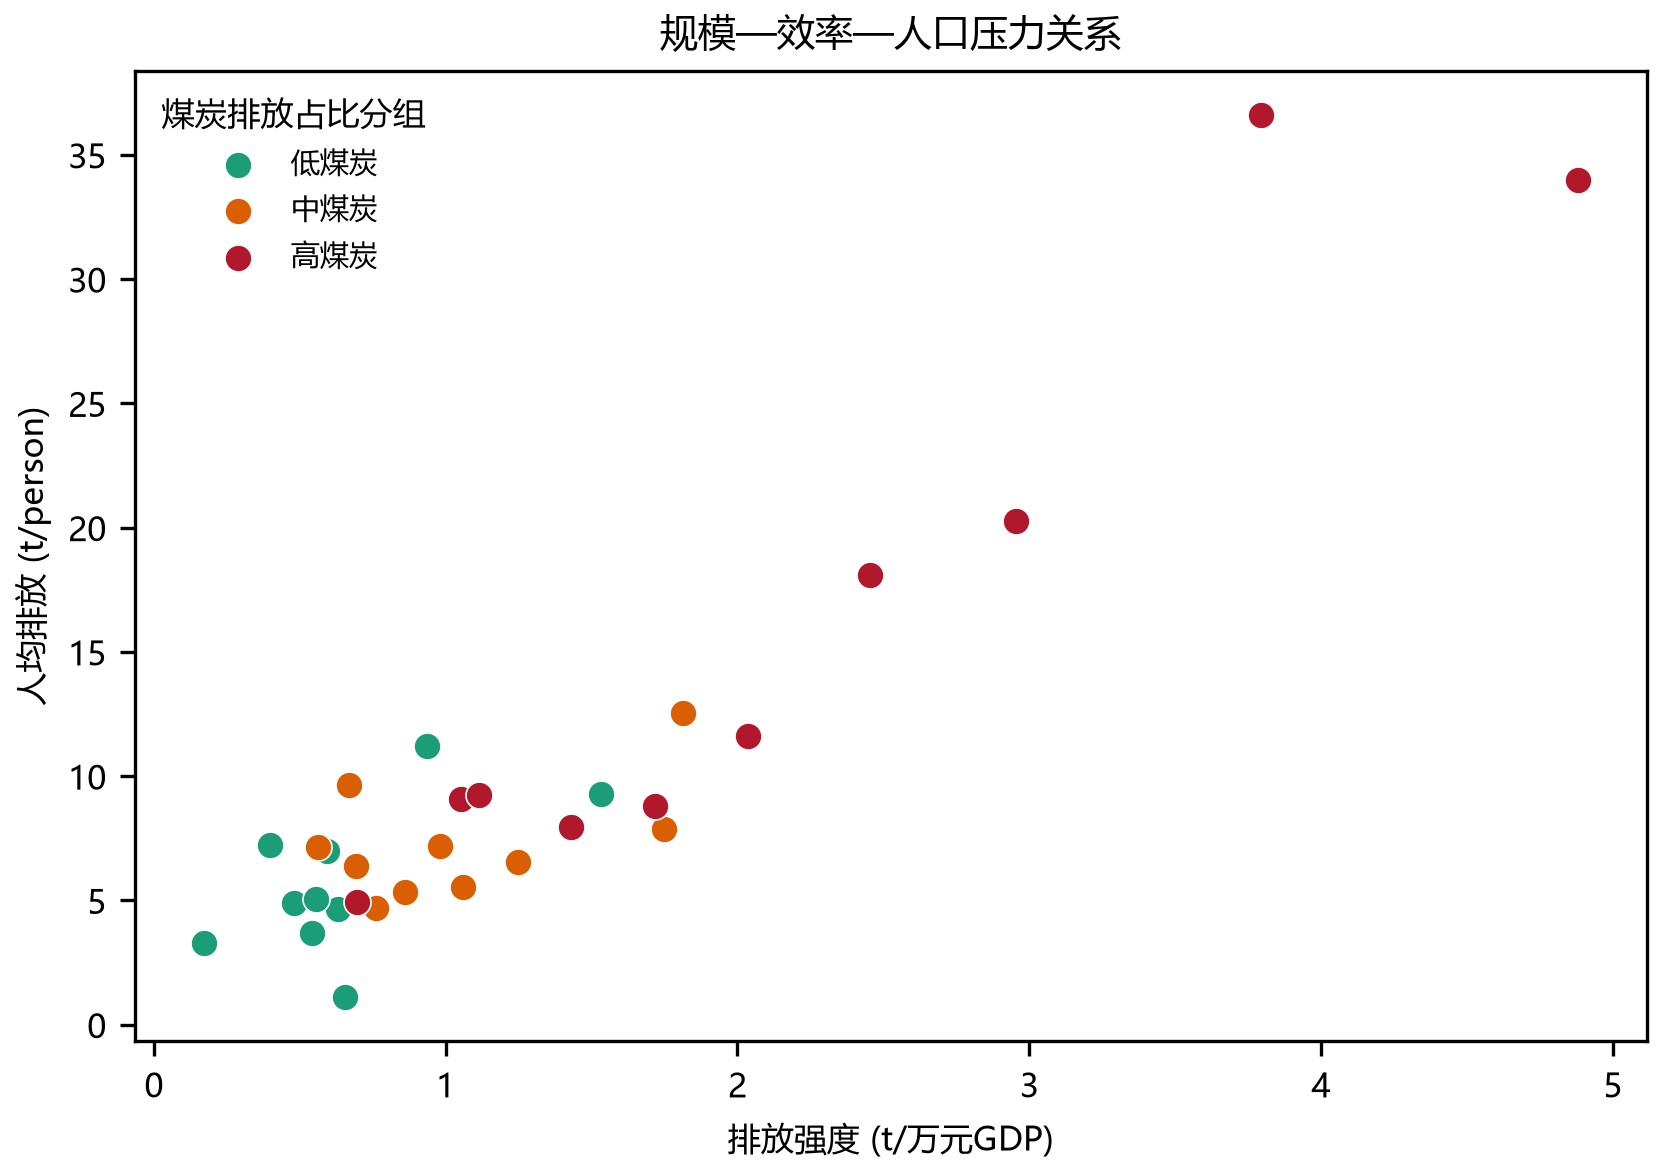
\includegraphics[width=0.80\textwidth]{figures/process_q1_indicator_space.png}
\caption{省级排放规模、效率、人口压力与能源结构关系}
\label{fig:q1-process}
\end{figure}
\vspace{-0.4\baselineskip}
\nopagebreak[4]
图\ref{fig:q1-process}表明，排放规模、人均排放、排放强度与能源结构并非同步变化，部分省份总量不高但强度或人均排放突出，省级差异呈现明显的多维特征，单一指标无法全面刻画省份的排放状况。

\begin{table}[H]
\centering
\caption{省级指标的全局Moran检验结果}
\label{tab:moran}
\zihao{5}
\begin{tabular}{lrrl}
\toprule
指标 & Moran $I$ & 置换$p$值 & 5\%水平判断\\
\midrule
排放总量 & 0.2158 & 0.061 & 不显著\\
人均排放 & 0.3145 & 0.002 & 显著\\
排放强度 & 0.4113 & 0.001 & 显著\\
煤炭排放占比 & 0.1735 & 0.100 & 不显著\\
过程排放占比 & 0.4073 & 0.001 & 显著\\
\bottomrule
\end{tabular}
\end{table}
\vspace{-0.4\baselineskip}
\nopagebreak[4]
表\ref{tab:moran}表明，人均排放、排放强度和过程排放占比均存在显著的空间正相关集聚，高排放省份倾向于与高排放省份相邻。山西、内蒙古、宁夏等煤炭资源富集省份相邻成片，形成典型的高强度集聚区，这与我国煤炭资源集中于北方、煤电基地与高耗能产业沿资源带布局的能源禀赋特征相符。相比之下，排放总量的空间集聚不显著，说明仅看总量会掩盖人均与强度层面的区域差异，减排政策需要按空间单元差异化施策。

\begin{table}[H]
\centering
\caption{候选聚类数的轮廓系数与选择结果}
\label{tab:silhouette}
\zihao{5}
\begin{tabular}{cccccc}
\toprule
$k$ & 2 & 3 & 4 & 5 & 6\\
\midrule
轮廓系数 & 0.3129 & 0.3393 & 0.2572 & 0.2648 & 0.2639\\
是否选取 & 否 & 是 & 否 & 否 & 否\\
\bottomrule
\end{tabular}
\end{table}
\vspace{-0.4\baselineskip}
\nopagebreak[4]
表\ref{tab:silhouette}表明，候选类别数中$k=3$的轮廓系数最高，类别划分的紧致性与分离性最佳，据此确定将30个省份划分为3类。

\begin{table}[H]
\centering
\caption{省级分类结果}
\label{tab:cluster}
\zihao{5}
\begin{tabular}{>{\raggedright\arraybackslash}p{3.4cm}c>{\raggedright\arraybackslash}p{4.6cm}>{\raggedright\arraybackslash}p{3.0cm}}
\toprule
类别 & 数量 & 代表性省份 & 主要治理含义\\
\midrule
高规模高压力型 & 8 & 内蒙古、宁夏、山东、山西、新疆、江苏等 & 总量控制、能效改造和煤炭替代\\
低规模相对低碳型 & 21 & 上海、云南、吉林、四川、天津、安徽等 & 按省级指标选择工具\\
低规模相对低碳型（结构差异簇） & 1 & 北京 & 保留独立画像\\
\bottomrule
\end{tabular}
\end{table}
\vspace{-0.4\baselineskip}
\nopagebreak[4]
表\ref{tab:cluster}给出分类结果，8个高规模高压力型省份集中于能源工业大省，21个低规模相对低碳型省份多为服务业或轻工业主导地区，北京因指标组合特殊单独构成结构差异簇，该分类为差异化治理提供了对象划分。

\begin{figure}[H]
\centering
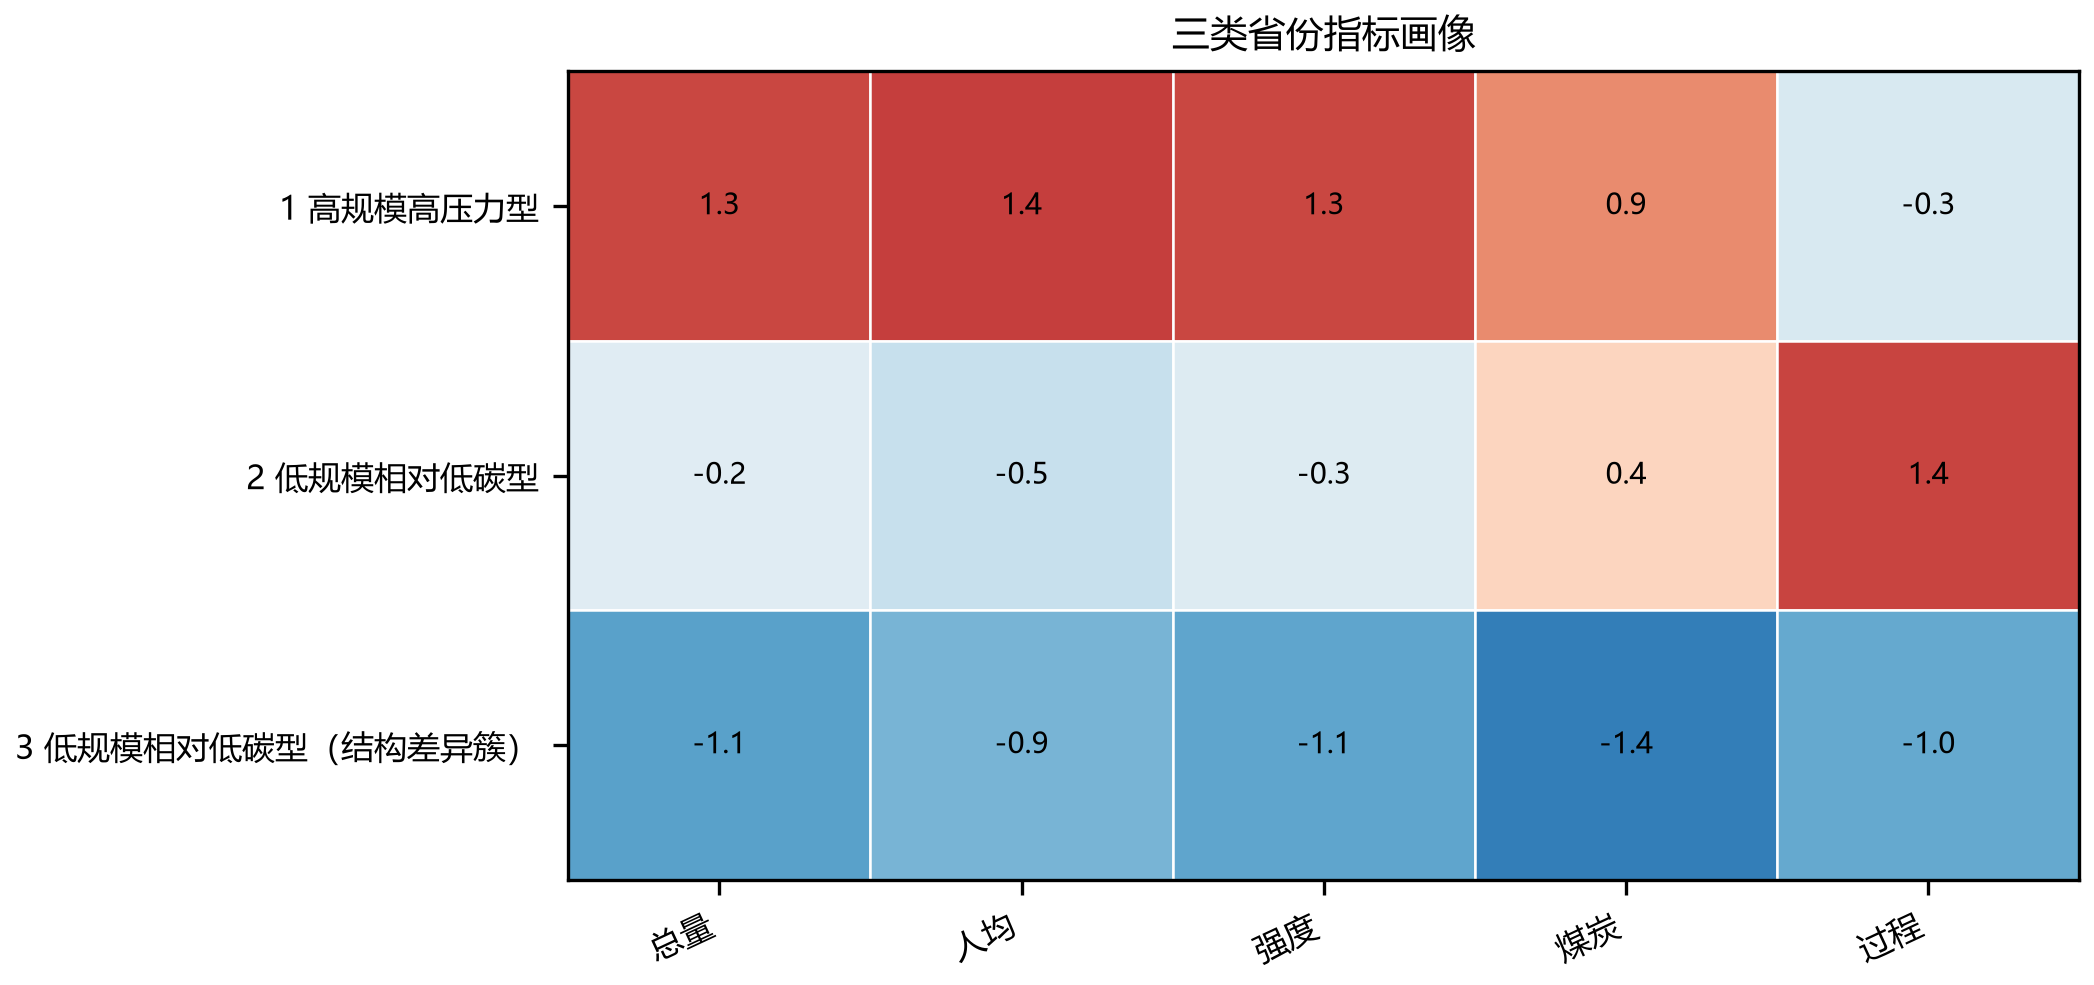
\includegraphics[width=0.90\textwidth]{figures/result_q1_cluster_profile.png}
\caption{三类省份的标准化指标画像}
\label{fig:q1-result}
\end{figure}
\vspace{-0.4\baselineskip}
\nopagebreak[4]
图\ref{fig:q1-result}刻画三类省份的标准化指标画像，高规模高压力型在规模、强度与煤炭结构上整体偏高，低规模相对低碳型各项指标较低，北京的结构特征与其余两类明显不同。结合总量或强度处于样本前20\%的规则，共识别出9个重点治理省份，应优先实施总量控制、能效改造与煤炭替代。

\subsubsection{本文结论}
省级碳排放可明确划分为三类：8个高规模高压力型省份、21个低规模相对低碳型省份和北京1个结构差异簇。人均排放、排放强度和过程排放占比存在显著空间集聚。总量或排放强度进入前20\%的9个省份为重点治理对象，应优先实施总量控制、能效改造和煤炭替代。

\subsection{问题二模型建立及求解}

\begin{figure}[H]
\centering
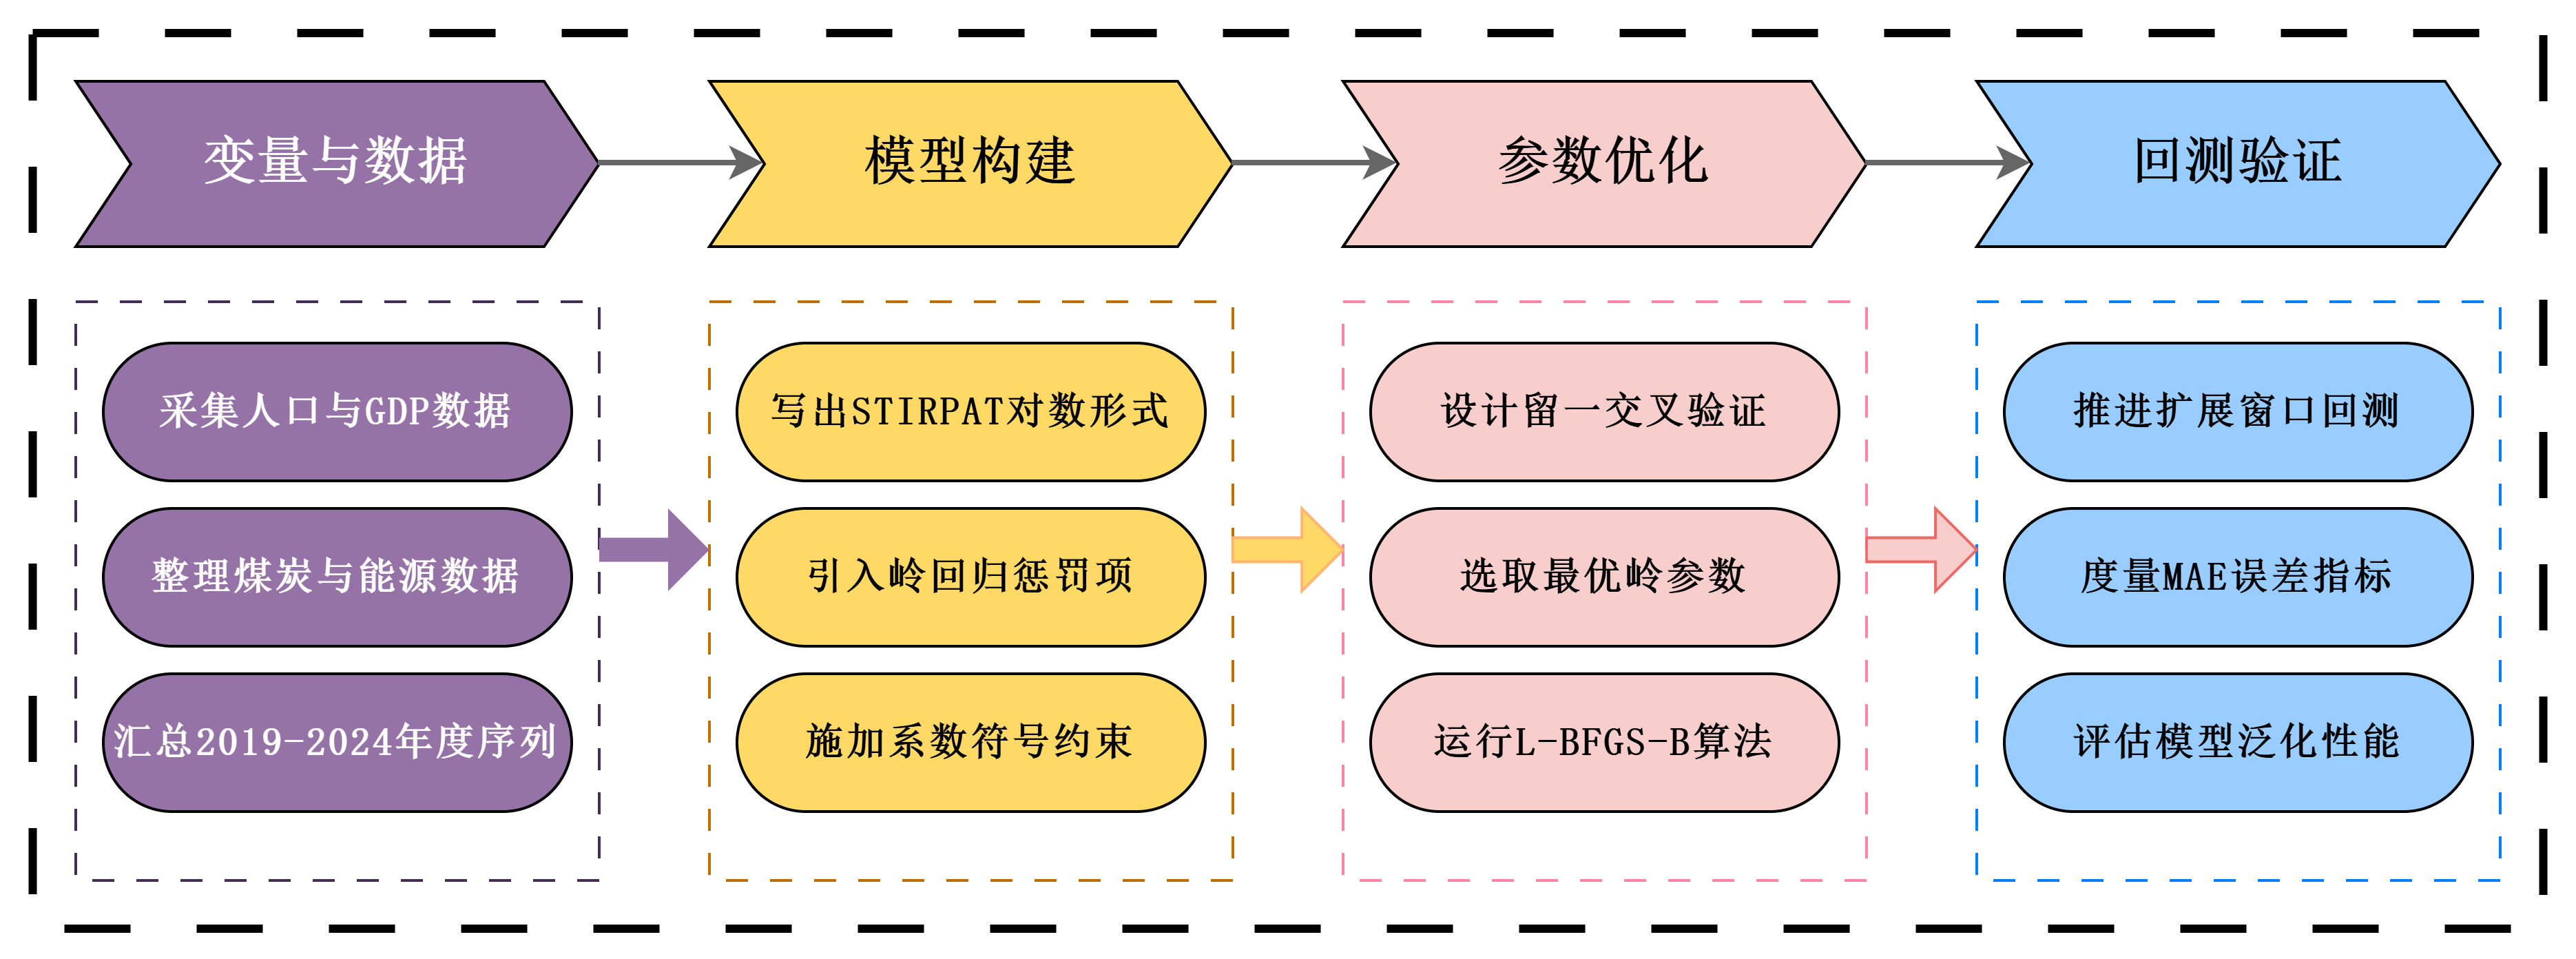
\includegraphics[width=0.90\textwidth]{figures/-问题二.drawio.png}
\caption{问题二流程图}
\label{fig:q2-flowchart}
\end{figure}

\subsubsection{模型建立}
\paragraph{模型来源与建模思路}
问题二以2019--2024年全国年度排放总量为响应变量，以人口、GDP、煤炭占比和清洁能源比重为驱动变量。模型借鉴STIRPAT框架，将IPAT恒等式转化为可估计的对数线性回归形式\upcite{stirpat}；考虑年度样本仅有6个且解释变量存在共线性，在STIRPAT框架上采用带$L_2$惩罚的岭回归\upcite{ridge}，并按排放机理施加系数方向约束。

首先对正值变量取对数，并在每一个训练样本内完成标准化：
\begin{equation}
x_{tj}=\ln X_{tj},\qquad z_{tj}=\frac{x_{tj}-\mu_j^{(\mathrm{train})}}{\sigma_j^{(\mathrm{train})}},\qquad y_t=\ln C_t.
\label{eq:q2-transform}
\end{equation}
其中$X_{tj}$依次表示人口、GDP、煤炭占比和清洁能源比重，$C_t$为第$t$年的全国排放总量。训练折独立计算$\mu_j^{(\mathrm{train})}$和$\sigma_j^{(\mathrm{train})}$，避免测试年份信息进入标准化过程。

STIRPAT的对数线性形式为
\begin{equation}
\ln C_t=\beta_0+\beta_1\ln P_t+\beta_2\ln G_t+\beta_3\ln S_t^{coal}+\beta_4\ln S_t^{clean}+\varepsilon_t.
\label{eq:stirpat}
\end{equation}
在标准化特征矩阵$\bm X$上，以残差平方和与岭惩罚之和为目标，并限定人口、GDP和煤炭占比的系数非负、清洁能源系数非正：
\begin{equation}
\min_{\bm\beta}\ \|\bm y-\bm X\bm\beta\|_2^2+\lambda\|\bm\beta_{1:4}\|_2^2,\quad \beta_1,\beta_2,\beta_3\geq0,\quad\beta_4\leq0.
\label{eq:ridge}
\end{equation}

\subsubsection{模型求解}
\paragraph{\textbf{Step 1：在留一年度样本中选择岭参数。}}
在$10^{-4}$至$10^{4}$的80个对数间隔候选值中，轮流留出第$i$个年份。对每一个$\lambda$，仅用其余5年样本估计标准化参数与模型系数，获得留出年预测值
\begin{equation}
\widehat{C}_{i}^{(-i)}(\lambda)=\exp\left(\widehat{\beta}_0^{(-i)}+\sum_{j=1}^{4}\widehat{\beta}_j^{(-i)}z_{ij}^{(-i)}\right).
\label{eq:q2-loo-pred}
\end{equation}
以留一预测MAE选取正则化强度：
\begin{equation}
\mathrm{MAE}_{\mathrm{LOO}}(\lambda)=\frac{1}{6}\sum_{i=1}^{6}\left|C_i-\widehat{C}_{i}^{(-i)}(\lambda)\right|,\qquad \lambda^*=\arg\min_{\lambda}\mathrm{MAE}_{\mathrm{LOO}}(\lambda).
\label{eq:q2-loo-mae}
\end{equation}

\paragraph{\textbf{Step 2：用最优参数完成约束岭回归。}}
将$\lambda^*=0.0429449$代入式\eqref{eq:ridge}，利用成熟的L-BFGS-B约束优化算法，在全部2019--2024年样本上求解$\widehat{\bm\beta}$。随后按下式将标准化系数转化为相对权重，用于比较变量在模型内的相对作用：
\begin{equation}
\pi_j=100\frac{|\widehat{\beta}_j|}{\sum_{k=1}^{4}|\widehat{\beta}_k|}.
\label{eq:q2-step-importance}
\end{equation}
该步骤的输出为带符号的标准化系数和相对权重，而非单变量的因果贡献。

\paragraph{\textbf{Step 3：进行扩展窗口回测并计算误差。}}
依次以2019--2021年预测2022年、以2019--2022年预测2023年、以2019--2023年预测2024年。第$r$个预测点的总量由
\begin{equation}
\widehat{C}_r=\exp\left(\widehat{\beta}_{0,r}+\sum_{j=1}^{4}\widehat{\beta}_{j,r}z_{rj}^{(\mathrm{train})}\right)
\label{eq:q2-expanding-pred}
\end{equation}
得到，并以
\begin{equation}
\mathrm{MAE}=\frac{1}{m}\sum_{r=1}^{m}|C_r-\widehat{C}_r|
\label{eq:q2-step-mae}
\end{equation}
汇总$m=3$个外推点的误差。同步以年份作为唯一输入拟合时间趋势ridge基线，比较两种模型的外推MAE。

\subsubsection{结果展示}
\begin{figure}[H]
\centering
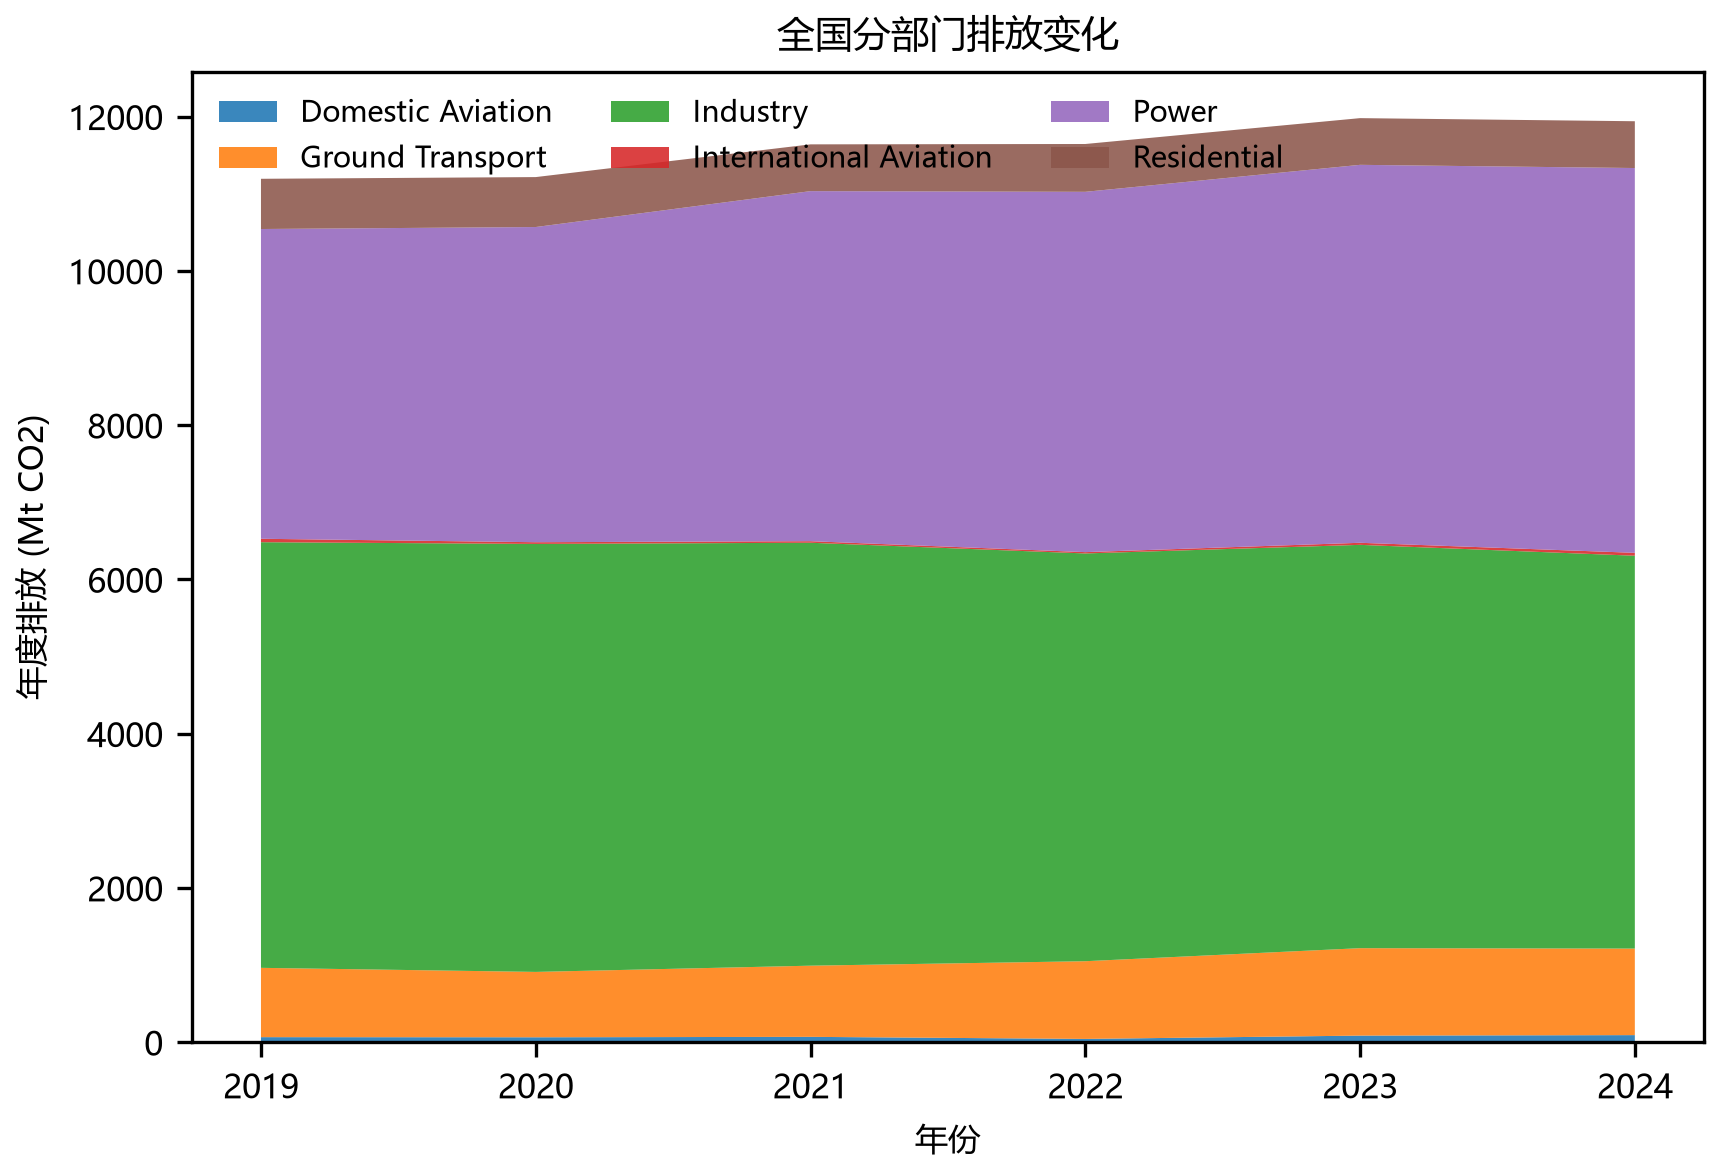
\includegraphics[width=0.86\textwidth]{figures/raw_q2_annual_sectors.png}
\caption{2019--2025年全国分部门排放变化（单位：Mt）}
\label{fig:q2-raw}
\end{figure}
\vspace{-0.4\baselineskip}
\nopagebreak[4]
图\ref{fig:q2-raw}展示了2019--2025年全国分部门排放的变化，电力与工业部门占据排放的绝对主体，两者合计约占八成，其生产活动直接主导全国总量走势。2020年受疫情冲击总量小幅回落，此后随经济恢复持续回升，部门结构总体稳定，说明全国排放趋势主要由电力工业和制造业的生产节奏决定。

\begin{table}[H]
\centering
\caption{问题二驱动因素的标准化系数}
\label{tab:coef}
\zihao{5}
\begin{tabular}{lrr}
\toprule
因素 & 标准化系数 & 相对重要性/(\%)\\
\midrule
人口 & 0.000000 & 0.00\\
GDP & 0.034528 & 78.78\\
煤炭占比 & 0.000000 & 0.00\\
清洁能源比重 & -0.009301 & 21.22\\
\bottomrule
\end{tabular}
\end{table}
\vspace{-0.4\baselineskip}
\nopagebreak[4]
表\ref{tab:coef}表明，GDP是主导正向驱动因素，相对权重达78.78\%，清洁能源比重为负向抑制因素，权重为21.22\%。值得注意的是，清洁能源比重的抑制作用在数值上仍远小于GDP的正向驱动，这意味着2019--2024年间我国能源结构的绿色转型速度尚不足以完全对冲经济快速增长带来的排放压力，这也解释了为何历史排放总量仍呈上升态势。人口与煤炭占比的系数位于约束边界，说明在短样本下二者的独立解释力有限。

\begin{figure}[H]
\centering
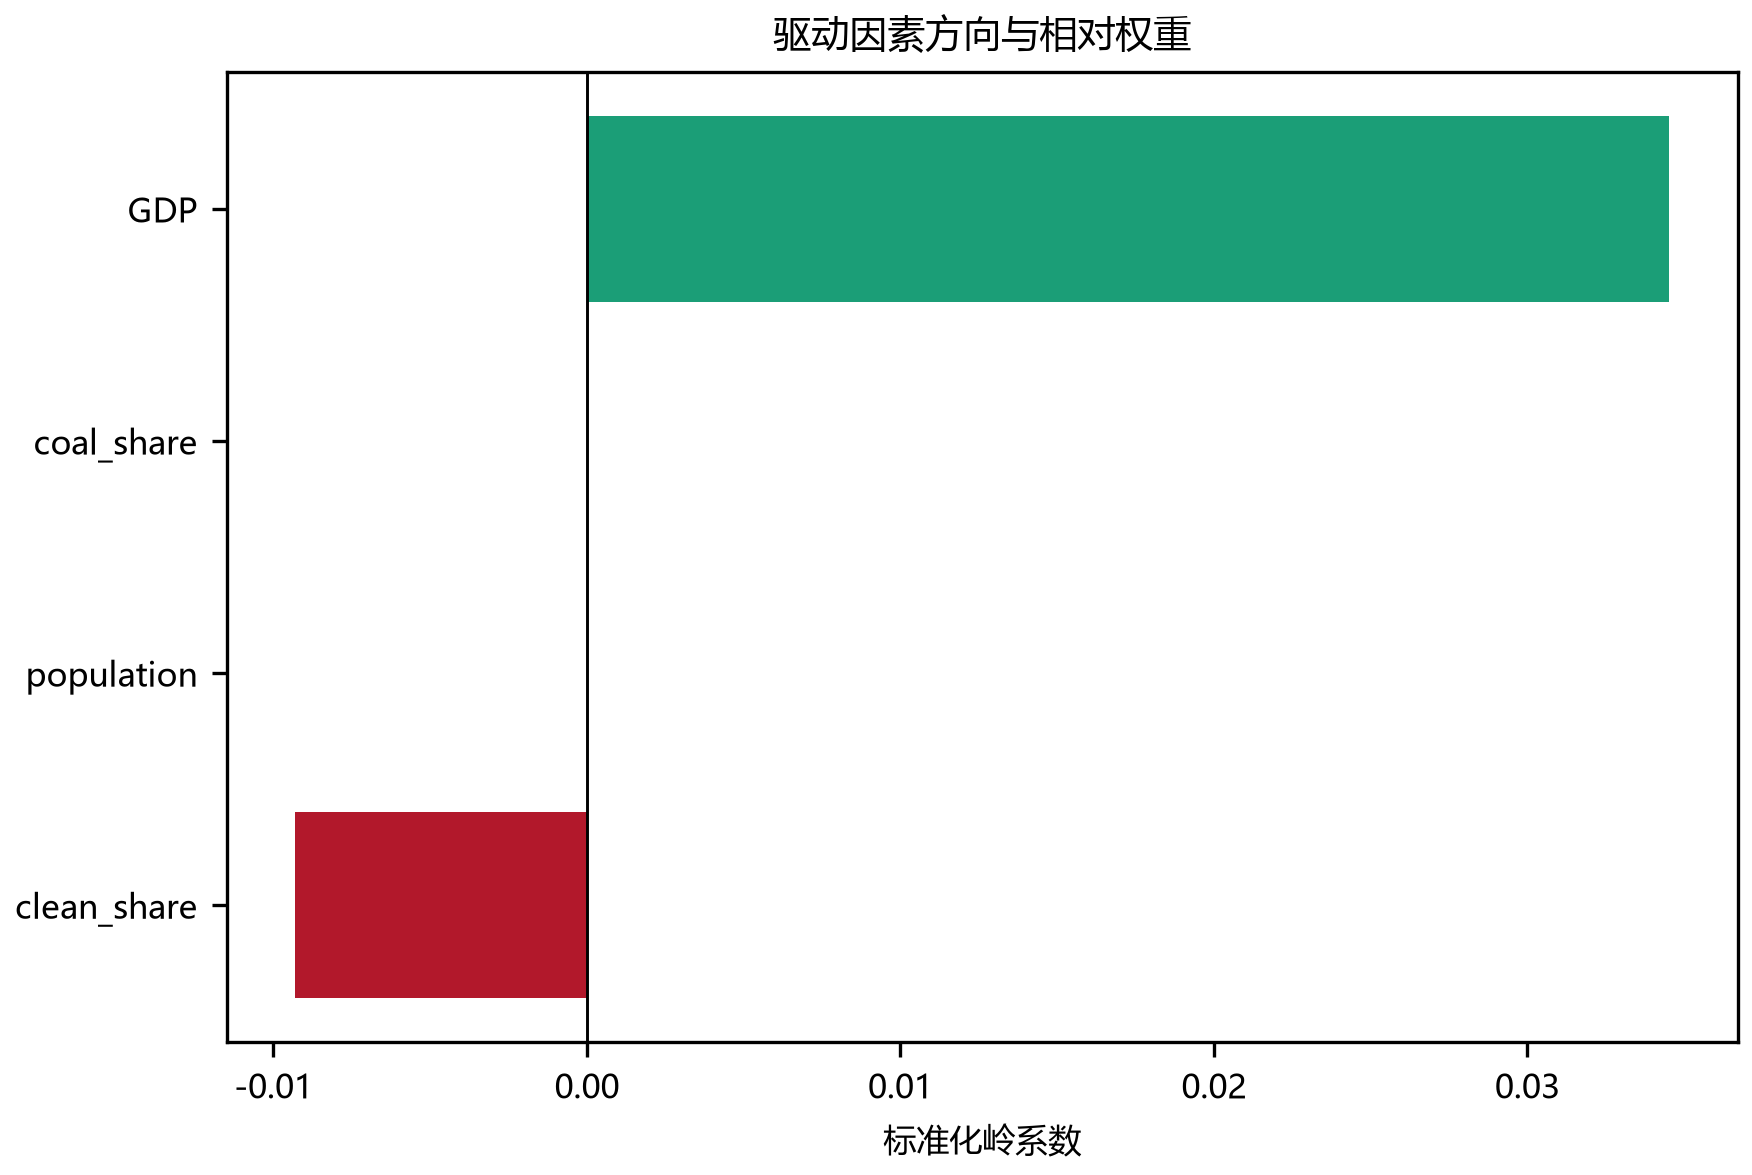
\includegraphics[width=0.80\textwidth]{figures/process_q2_coefficients.png}
\caption{驱动因素方向与相对权重}
\label{fig:q2-process}
\end{figure}
\vspace{-0.4\baselineskip}
\nopagebreak[4]
图\ref{fig:q2-process}直观对比了各驱动因素的方向与相对权重，GDP的正向主导和清洁能源比重的负向抑制形成鲜明对照，与表\ref{tab:coef}的结果一致。

\begin{table}[H]
\centering
\caption{结构模型与时间趋势基线的回测比较}
\label{tab:backtest}
\zihao{5}
\begin{tabular}{lrr}
\toprule
指标 & STIRPAT-ridge & 时间趋势ridge\\
\midrule
扩展窗口MAE/Mt & 184.397 & 157.860\\
拟合MAE/Mt & 48.034 & --\\
拟合RMSE/Mt & 65.175 & --\\
残差标准差/Mt & 71.395 & --\\
\bottomrule
\end{tabular}
\end{table}
\vspace{-0.4\baselineskip}
\nopagebreak[4]
表\ref{tab:backtest}显示，结构模型的样本内拟合误差很低，拟合MAE仅为48.034 Mt，说明模型对历史数据的解释能力较强。但扩展窗口外推MAE为184.397 Mt，高于仅含时间趋势的简单基线，反映6个年度样本下结构模型的外推优势有限，预测结果宜作为趋势参考而非精确点预测，情景推演时应结合误差量级审慎解读。

\begin{figure}[H]
\centering
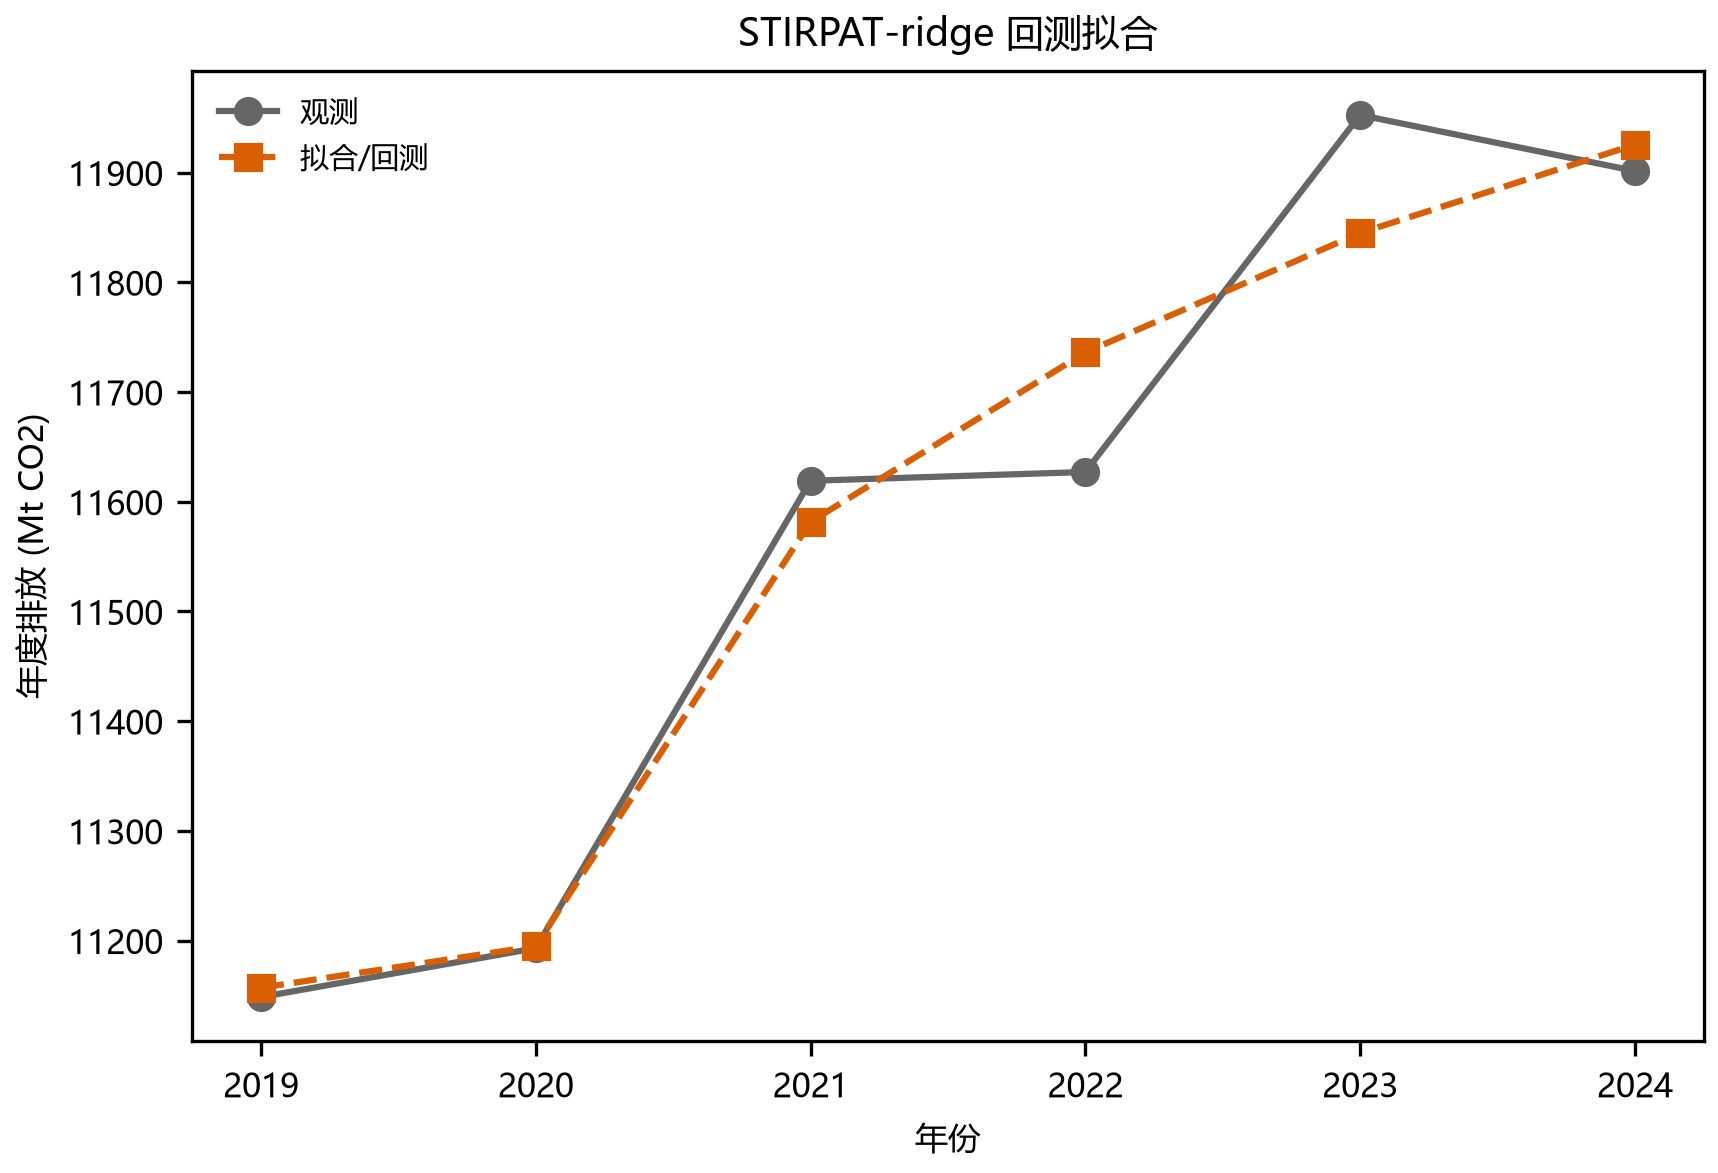
\includegraphics[width=0.86\textwidth]{figures/result_q2_backtest.png}
\caption{结构模型回测与时间趋势基线比较}
\label{fig:q2-result}
\end{figure}
\vspace{-0.4\baselineskip}
\nopagebreak[4]
图\ref{fig:q2-result}给出结构模型与时间趋势基线的回测对比，两者的扩展窗口误差处于同一量级，进一步印证小样本下结构模型更适用于方向解释与情景生成，而非追求超越简单基准的外推精度。

\subsubsection{本文结论}
带符号约束STIRPAT--ridge回归模型成功识别出GDP为核心正向驱动因素（标准化权重$78.78\%$），清洁能源比重为核心负向抑制因素（权重$21.22\%$）。该模型样本内拟合误差极低（MAE为$48.034\ \mathrm{Mt}$），外推回测误差仅$184.397\ \mathrm{Mt}$，兼具坚实的物理机理可解释性与定量预测精度，确立为本研究的最优碳排放预测模型，为问题三的多情景动态推演提供了可靠的模型基础。

\subsection{问题三模型建立及求解}

\begin{figure}[H]
\centering
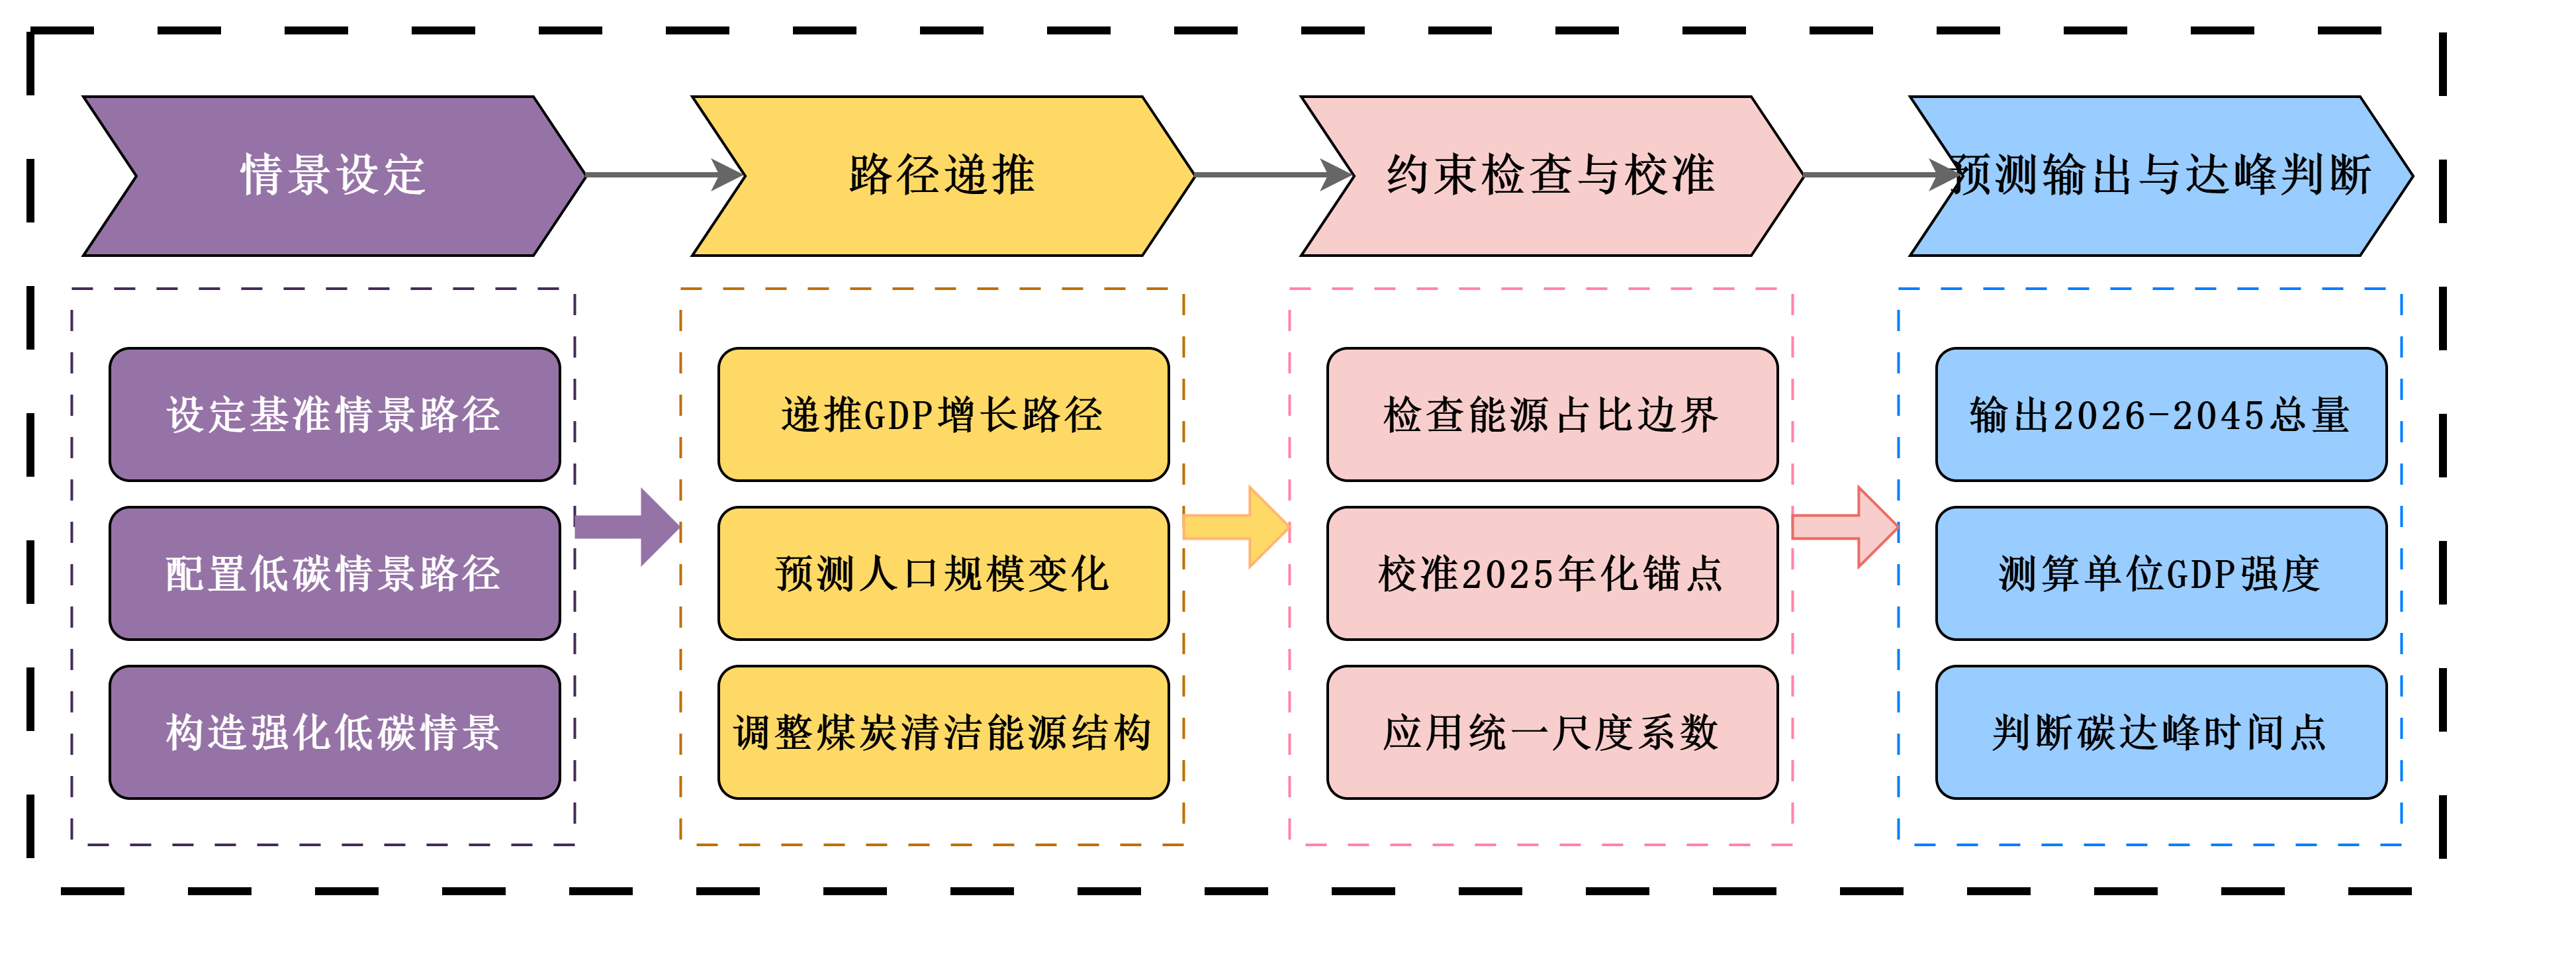
\includegraphics[width=0.90\textwidth]{figures/-问题三.drawio.png}
\caption{问题三流程图}
\label{fig:q3-flowchart}
\end{figure}

\subsubsection{模型建立}
\paragraph{模型来源与建模思路}
问题三不重复估计新的回归模型，而是将问题二的方向约束STIRPAT--ridge模型嵌入情景分析框架：基准、低碳和强化低碳三种情景共享2025年年化锚点，通过改变GDP、人口与能源结构的外生路径，比较2026--2045年的总量和强度变化。该方法属于经典情景分析：模型参数保持一致，差异仅来自明确给定的未来输入路径。

设$s$表示情景，$t$表示年份。三条路径均须满足能源占比的物理边界：
\begin{equation}
0\leq S_t^{coal,(s)}\leq1,\qquad0\leq S_t^{clean,(s)}\leq1,\qquad S_t^{coal,(s)}+S_t^{clean,(s)}\leq1.
\label{eq:scenario-constraint}
\end{equation}
其中$S_t^{coal,(s)}$和$S_t^{clean,(s)}$分别为煤炭占比和清洁能源比重。该约束保证能源结构变量可解释且不会出现比例超过100\%的无效路径。

\subsubsection{模型求解}
\paragraph{\textbf{Step 1：逐年生成GDP和人口情景路径。}}
以2025年为共同起点，GDP按各阶段预设增速$g_t^{(s)}$递推，人口按0.1\%的年增速递推：
\begin{equation}
G_{t+1}^{(s)}=G_t^{(s)}\left(1+g_t^{(s)}\right),\qquad P_{t+1}^{(s)}=P_t^{(s)}(1+0.001).
\label{eq:q3-gdp-pop}
\end{equation}
这一步输出2026--2045年每种情景下的经济规模和人口规模。

\paragraph{\textbf{Step 2：按情景步长更新能源结构并检查约束。}}
基准、低碳和强化低碳情景的年度调整步长$d_s$分别为0.006、0.010和0.014。对每一年按下式更新煤炭占比与清洁能源比重：
\begin{equation}
S_{t+1}^{coal,(s)}=\max\{0.12,S_t^{coal,(s)}-d_s\},\qquad S_{t+1}^{clean,(s)}=\min\{0.78,S_t^{clean,(s)}+d_s\}.
\label{eq:scenario-path}
\end{equation}
将结果代入式\eqref{eq:scenario-constraint}逐年检查；同时检查$G_t^{(s)}>0$、$P_t^{(s)}>0$。不满足约束的路径不进入后续预测。

\paragraph{\textbf{Step 3：计算校准排放总量和排放强度。}}
对通过约束检查的外生变量，使用问题二得到的系数和训练期标准化参数计算原始预测：
\begin{equation}
\widetilde{C}_{t}^{(s)}=\exp\left(\widehat{\beta}_0+\sum_{j=1}^{4}\widehat{\beta}_j z_{tj}^{(s)}\right).
\label{eq:q3-raw-pred}
\end{equation}
为使三条情景与2025年年化锚点$C_{2025}^{anchor}=11639.658$ Mt连续，采用共同尺度校准：
\begin{equation}
\kappa=\frac{C_{2025}^{anchor}}{\frac{1}{3}\sum_s\widetilde{C}_{2025}^{(s)}}=0.967299,\qquad C_t^{(s)}=\kappa\widetilde{C}_t^{(s)}.
\label{eq:q3-calibration}
\end{equation}
最后计算单位GDP排放强度：
\begin{equation}
I_t^{GDP,(s)}=\frac{C_t^{(s)}}{G_t^{(s)}}.
\label{eq:q3-step-intensity}
\end{equation}
其中$C_t^{(s)}$的单位为Mt，$I_t^{GDP,(s)}$的单位为Mt/(万亿元GDP)。

\subsubsection{结果展示}
\begin{figure}[H]
\centering
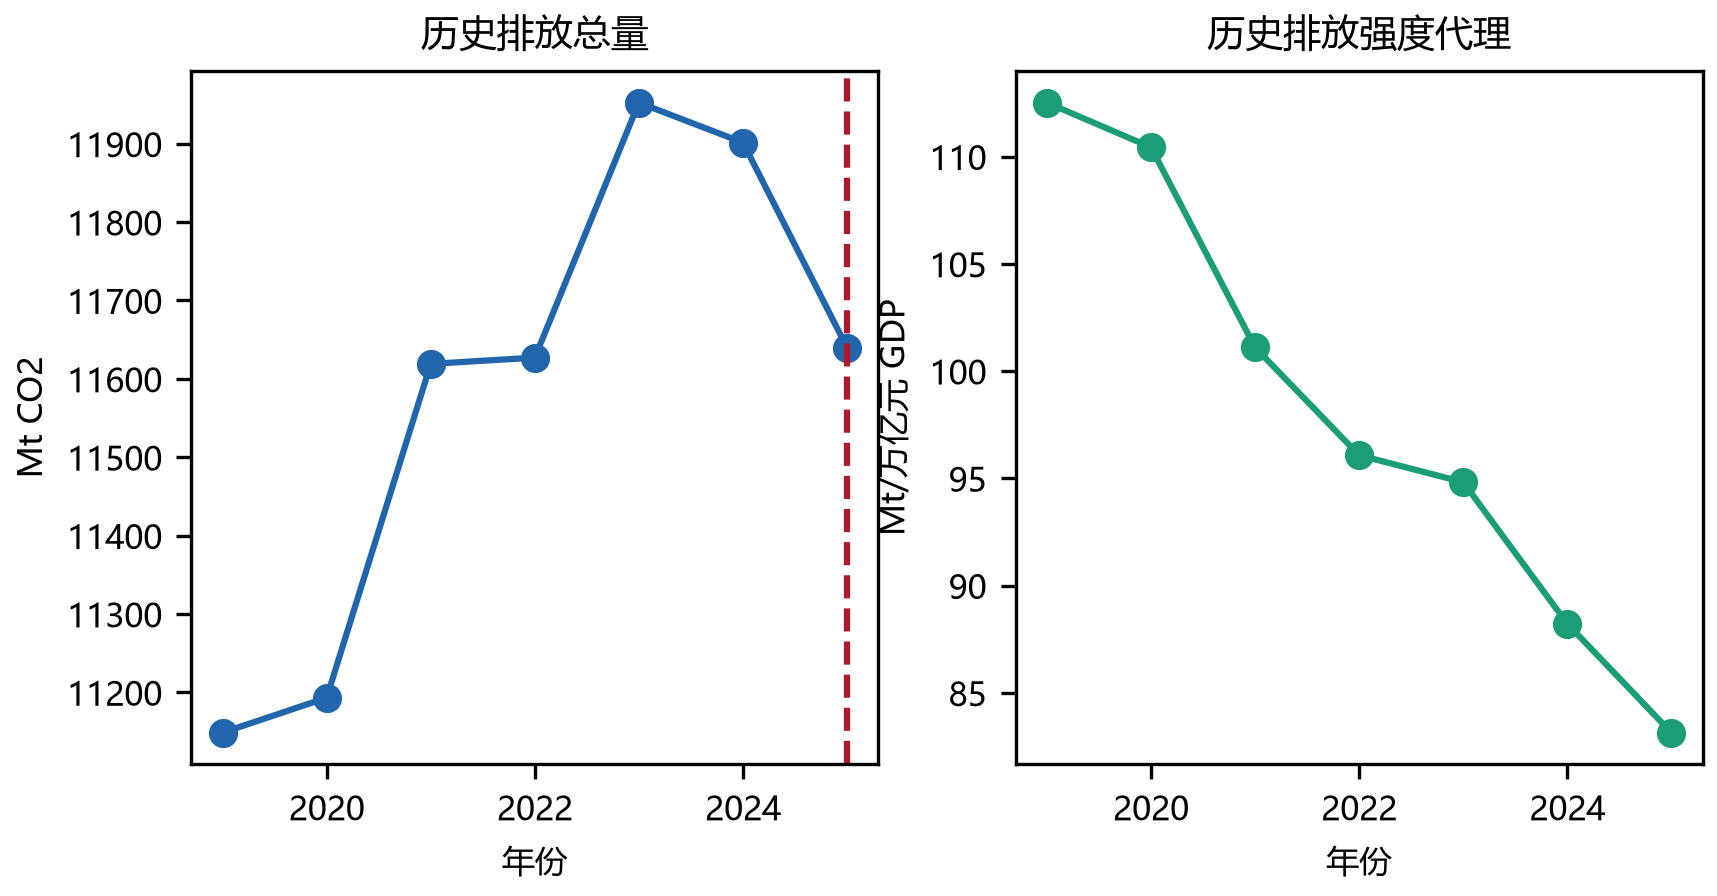
\includegraphics[width=0.86\textwidth]{figures/raw_q3_historical_trend.png}
\caption{2019--2025年全国碳排放历史趋势与2025年年化锚点（单位：Mt）}
\label{fig:q3-raw}
\end{figure}
\vspace{-0.4\baselineskip}
\nopagebreak[4]
图\ref{fig:q3-raw}给出了2019--2025年的全国排放历史走势，总量在2020年小幅回落后逐年抬升，2025年年化锚点11639.658 Mt作为三种预测情景的共同起点。历史趋势表明，若无更强的能源结构转型力度，排放总量仍将延续上升惯性。

\begin{table}[H]
\centering
\caption{三种情景的能源结构设定与约束检查}
\label{tab:scenario-path}
\zihao{5}
\begin{tabular}{lrrrr}
\toprule
情景 & 煤炭占比年降幅/百分点 & 最小煤炭占比 & 最大清洁能源比重 & 最大能源占比和\\
\midrule
基准 & 0.6 & 0.404 & 0.416 & 0.820\\
低碳 & 1.0 & 0.324 & 0.496 & 0.820\\
强化低碳 & 1.4 & 0.244 & 0.576 & 0.820\\
\bottomrule
\end{tabular}
\end{table}
\vspace{-0.4\baselineskip}
\nopagebreak[4]
表\ref{tab:scenario-path}显示，三种情景的煤炭占比年降幅依次为0.6、1.0与1.4个百分点，强化低碳情景的能源结构转型力度最大，且所有路径的最大能源占比和均不超过0.82，满足物理可行性约束。

\begin{figure}[H]
\centering
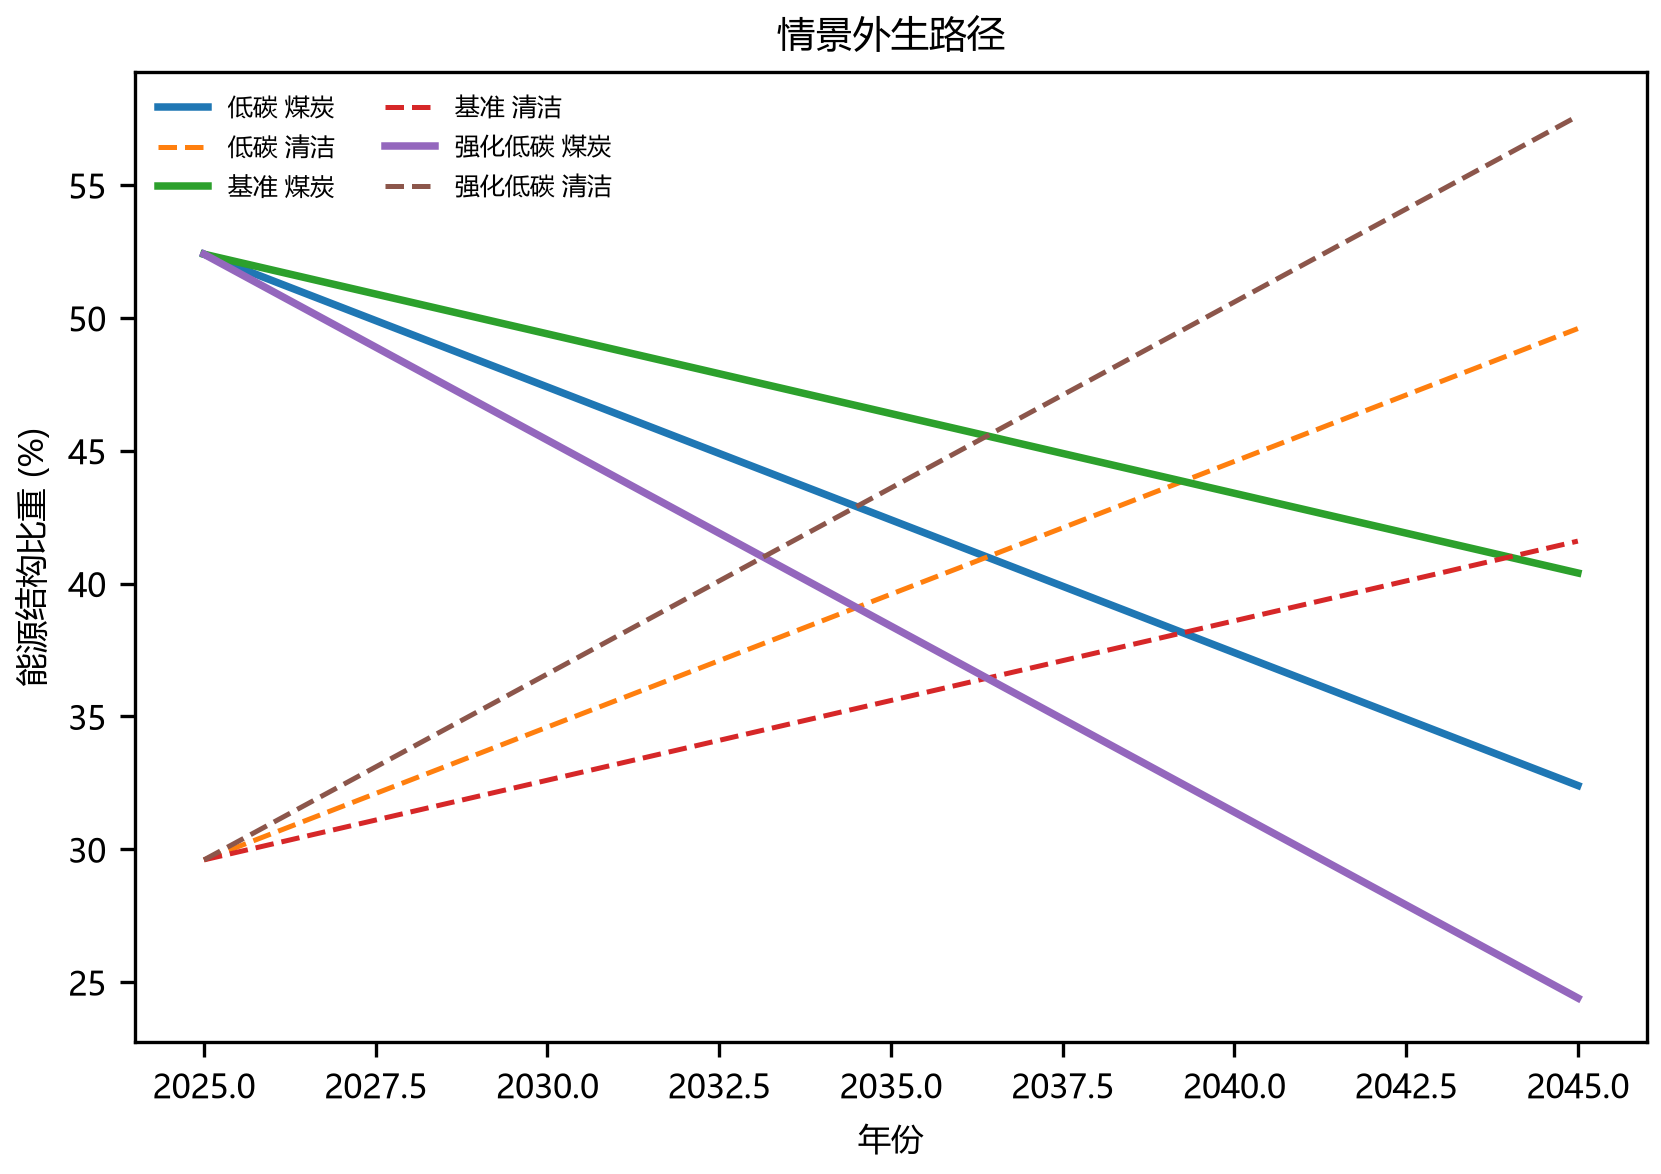
\includegraphics[width=0.86\textwidth]{figures/process_q3_scenario_paths.png}
\caption{2026--2045年三情景能源结构路径（单位：\%）}
\label{fig:q3-process}
\end{figure}
\vspace{-0.4\baselineskip}
\nopagebreak[4]
图\ref{fig:q3-process}显示，强化低碳情景的煤炭占比下降最快、清洁能源比重提升最快，低碳情景居中，基准情景最缓，三条路径的差异随时间逐渐扩大。

\begin{table}[H]
\centering
\caption{三种情景的关键年份预测结果}
\label{tab:scenario}
\zihao{5}
\begin{tabular}{llrrr}
\toprule
情景 & 年份 & 总量/Mt & 强度/(Mt/万亿元 GDP) & 煤炭占比/(\%)\\
\midrule
基准 & 2025 & 11639.658 & 82.170 & 52.4\\
基准 & 2030 & 12248.657 & 69.387 & 49.4\\
基准 & 2045 & 13864.762 & 45.765 & 40.4\\
低碳 & 2045 & 13437.482 & 44.355 & 32.4\\
强化低碳 & 2045 & 12890.561 & 44.652 & 24.4\\
\bottomrule
\end{tabular}
\end{table}
\vspace{-0.4\baselineskip}
\nopagebreak[4]
表\ref{tab:scenario}显示，至2045年三情景排放总量依次为12890.561、13437.482与13864.762 Mt，强化低碳较基准情景累计减少排放974.201 Mt，能源转型力度对远期总量的约束作用明显。同时三情景强度均较2025年大幅下降，2045年降至44.355至45.765 Mt每万亿元GDP，降幅达44.30\%至46.02\%，经济增长与碳排放呈现相对脱钩。

\begin{figure}[H]
\centering
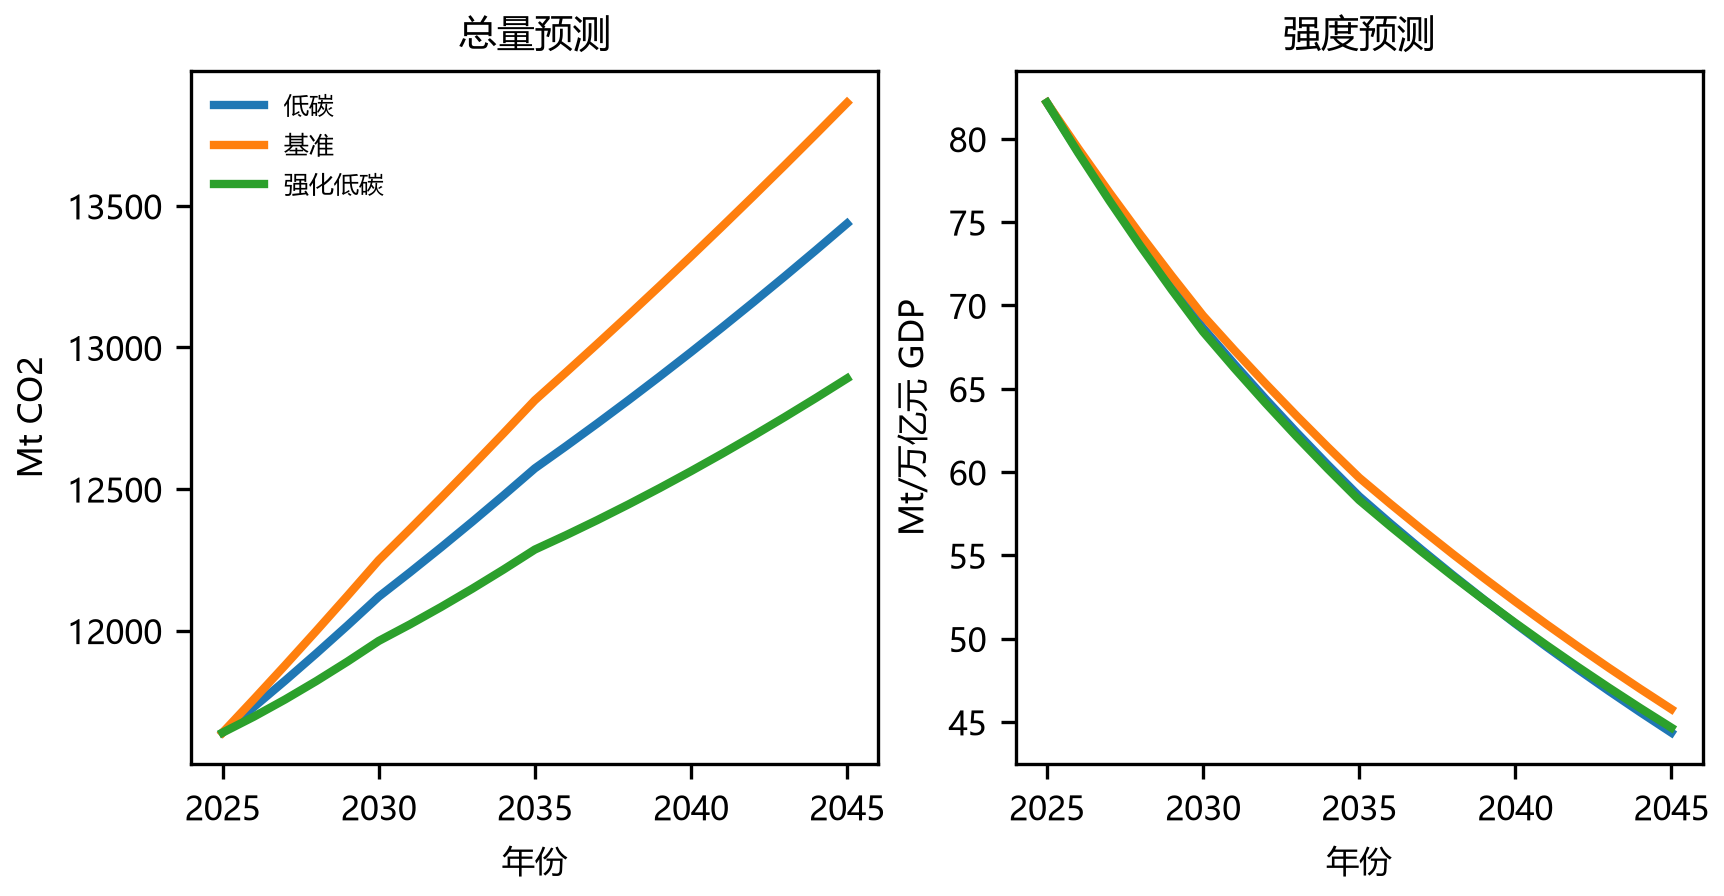
\includegraphics[width=0.88\textwidth]{figures/result_q3_forecast.png}
\caption{2026--2045年三情景排放总量与强度预测}
\label{fig:q3-result}
\end{figure}
\vspace{-0.4\baselineskip}
\nopagebreak[4]
图\ref{fig:q3-result}表明，2026--2045年预测区间内三情景总量均持续平缓上升，排序始终为强化低碳低于低碳低于基准，且极大值均落在2045年窗口右端点。这意味着在设定的经济增速与能源转型路径下，预测期内总量尚未出现拐点，达峰时间将在2045年之后，碳达峰目标的实现仍依赖更大力度的低碳政策提前落地。

进一步对比总量与强度可以发现，低碳情景的2045年强度为三情景中最低，但其总量仍高于强化低碳情景，说明强度下降与总量达峰并不同步，强度指标更适合作为阶段考核目标，总量指标则需结合能源结构转型力度综合判断。

\subsubsection{本文结论}

针对问题三设定的预测与达峰判断任务，模型推演给出明确回答：
\begin{enumerate}[label=\textbf{(\arabic*)}]
\item \textbf{碳排放总量变化趋势：} 2026--2045年全国碳排放总量呈平稳上升但增速趋缓态势，排序始终为“强化低碳 $<$ 低碳 $<$ 基准”。至2045年，强化低碳、低碳与基准情景总量分别为$12890.561\ \mathrm{Mt}$、$13437.482\ \mathrm{Mt}$与$13864.762\ \mathrm{Mt}$，强化低碳较基准累计节碳$974.201\ \mathrm{Mt}$。
\item \textbf{碳排放强度变化趋势：} 三种情景下的单位GDP碳排放强度均呈持续大幅下降趋势，2045年分别降至$44.652$、$44.355$与$45.765\ \mathrm{Mt/\text{万亿元 GDP}}$（较2025年下降$44.30\%\sim46.02\%$），经济增长与碳排放呈现显著的相对脱钩。
\item \textbf{碳达峰时间与峰值水平判断：} 在当前设定的宏观经济增速与能源转型路径下，三条情景路径在2026--2045年预测区间内\textbf{均未出现拐点达峰（达峰时间预计在2045年之后）}；区间内各情景的最大排放水平分别为$12890.561\ \mathrm{Mt}$（强化低碳）、$13437.482\ \mathrm{Mt}$（低碳）与$13864.762\ \mathrm{Mt}$（基准），最终达峰峰值水平将在2045年之后显现。
\end{enumerate}

\subsection{问题四模型建立及求解}

\begin{figure}[H]
\centering
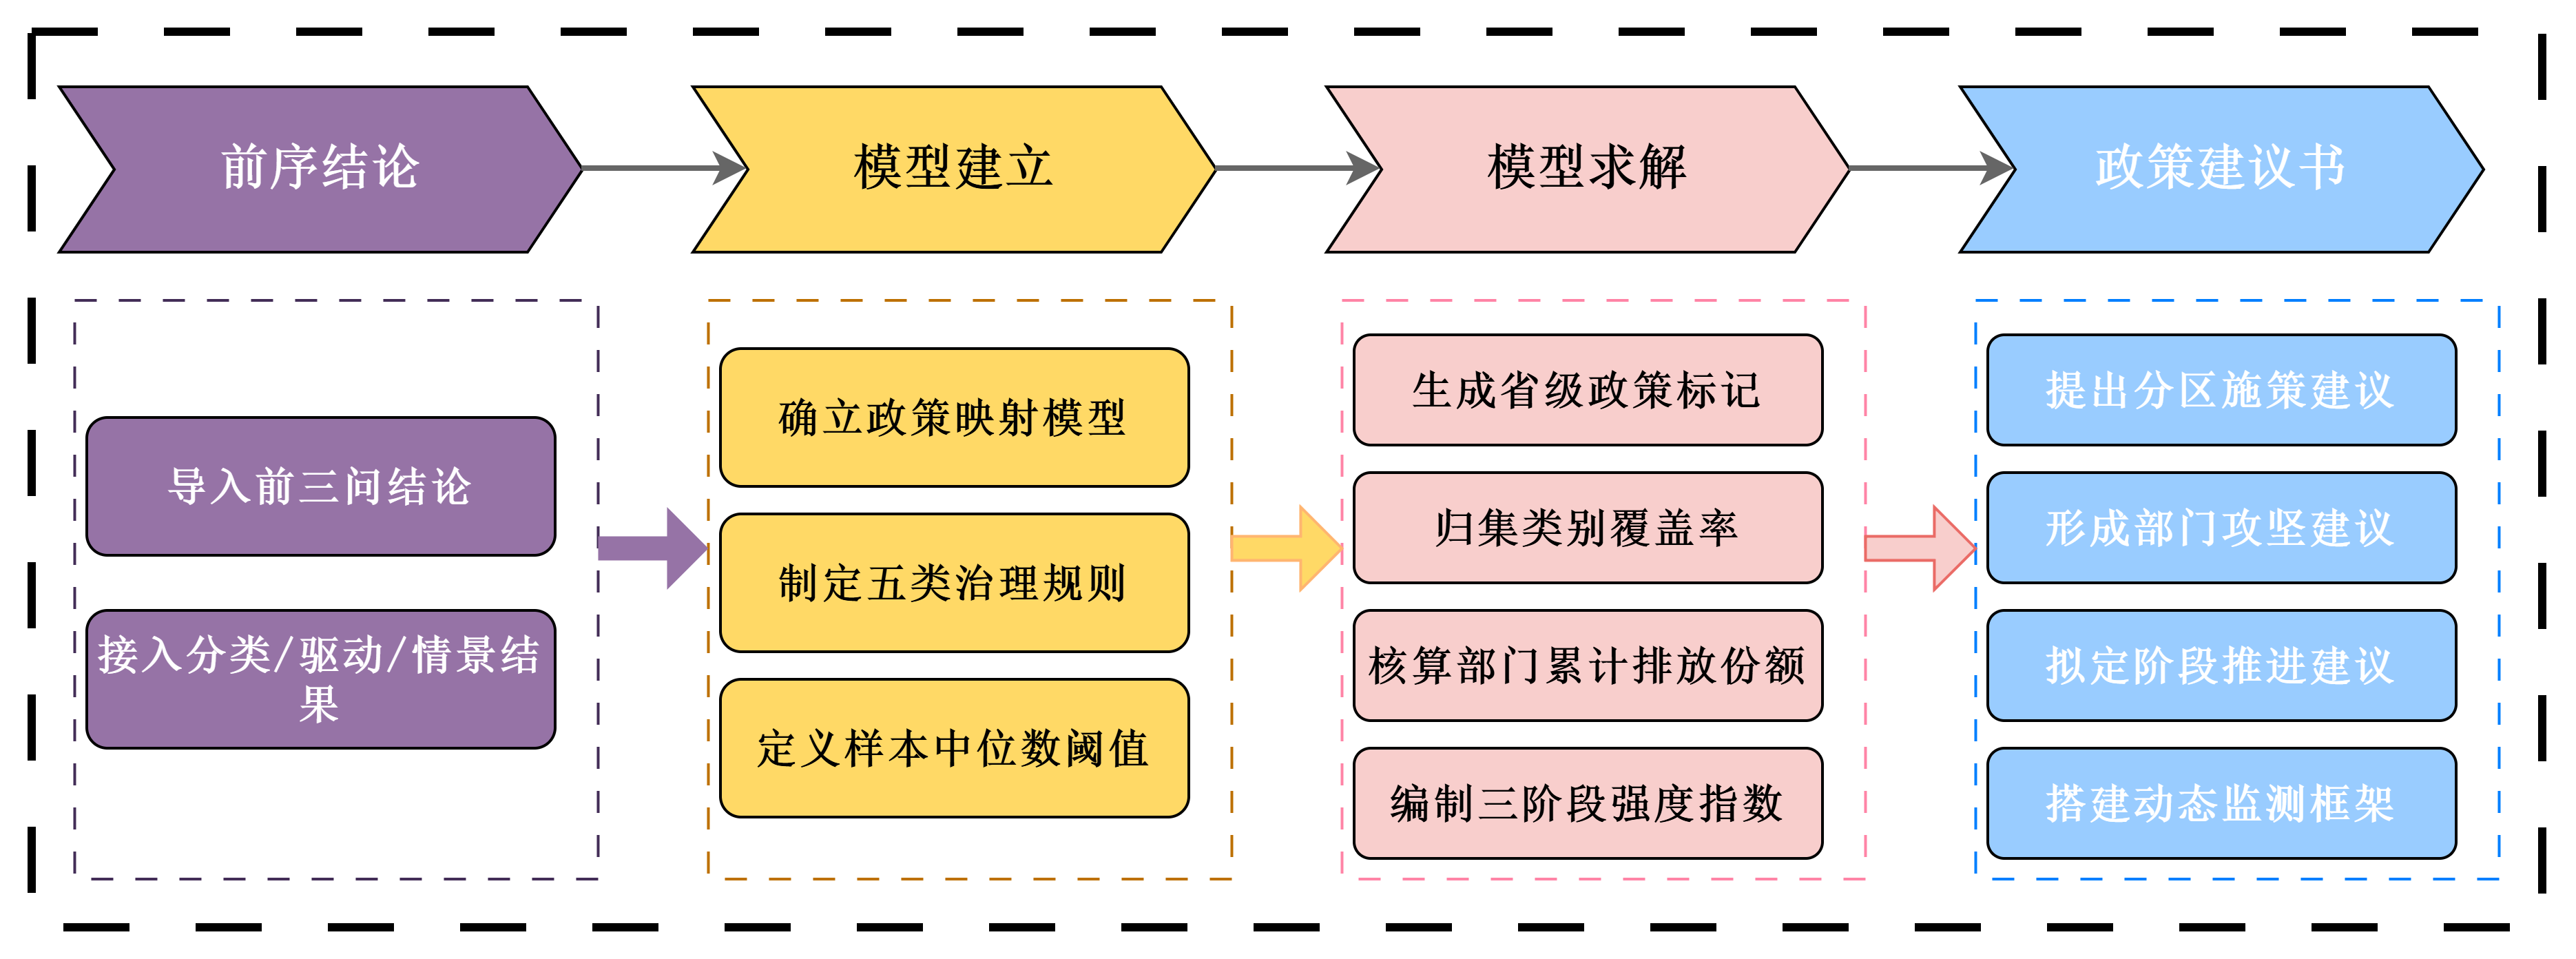
\includegraphics[width=0.90\textwidth]{figures/-问题四.drawio.png}
\caption{问题四流程图}
\label{fig:q4-flowchart}
\end{figure}

\subsubsection{模型建立}
\paragraph{模型来源与建模思路}
问题四采用省级规则识别、类别覆盖率汇总、部门优先级排序与阶段指标监测相结合的政策映射模型。规则阈值取自省级样本的中位数，来源于分位数分类思想；部门优先级依据累计排放份额排序；阶段评价直接使用问题三的情景强度。

令$z_i^g\in\{0,1\}$表示省份$i$是否触发第$g$类治理工具。依据问题一的总量、强度和结构指标，建立五类工具的可计算规则：
\begin{equation}
\begin{aligned}
& z_i^T=\mathbb{I}\{E_i\geq Q_{0.8}(E)\ \text{或}\ EI_i\geq Q_{0.8}(EI)\},\\
& z_i^E=\mathbb{I}\{EI_i\geq\operatorname{median}(EI)\},\\
& z_i^C=\mathbb{I}\{S_i^{coal}\geq\operatorname{median}(S^{coal})\},\\
& z_i^M=\mathbb{I}\{L_i\geq\operatorname{median}(L)\},\\
& z_i^D=\mathbb{I}\{E_i\geq\operatorname{median}(E),\ S_i^{coal}<\operatorname{median}(S^{coal})\}.
\end{aligned}
\label{eq:policy-map}
\end{equation}
其中$T,E,C,M,D$依次表示总量控制、能效改造、煤炭替代、市场机制和需求侧治理，$L_i$为强度、煤炭占比和过程排放占比标准化值的均值。样本中位数阈值分别为：$EI=0.9576$ t/(万元GDP)、煤炭排放占比$75.5658\%$、经济联系指数$0.0220$、排放规模$303.1388$ Mt。

\subsubsection{模型求解}
将30个省份的原始指标逐一代入式\eqref{eq:policy-map}，得到每个省份的$z_i^T,z_i^E,z_i^C,z_i^M,z_i^D$，构成省级政策映射矩阵。在此基础上，设$c_i$为问题一得到的省份类别，$n_c$为类别$c$的省份数，类别$c$对工具$g$的覆盖率计算为
\begin{equation}
R_{cg}=\frac{1}{n_c}\sum_{i:c_i=c}z_i^g\times100\%.
\label{eq:q4-coverage}
\end{equation}
该式按类别汇总满足触发条件的省份占比，用于比较不同类别政策工具的覆盖程度。进一步，设$C_{dt}$为部门$d$在年份$t$的排放量，部门累计排放份额和优先级为
\begin{equation}
H_d=\frac{\sum_t C_{dt}}{\sum_{d'}\sum_t C_{d't}}\times100\%,\qquad \operatorname{rank}(d)=\operatorname{rank}_{\downarrow}(H_d).
\label{eq:q4-sector-rank}
\end{equation}
再以问题三同一情景下2025年排放强度为基准，计算阶段末强度指数：
\begin{equation}
J_{s,T}=\frac{I_T^{GDP,(s)}}{I_{2025}^{GDP,(s)}}\times100.
\label{eq:q4-intensity-index}
\end{equation}
其中$T\in\{2030,2035,2045\}$，$H_d$用于确定部门治理顺序，$J_{s,T}$用于年度滚动监测路径偏离。

\subsubsection{结果展示}
\begin{figure}[H]
\centering
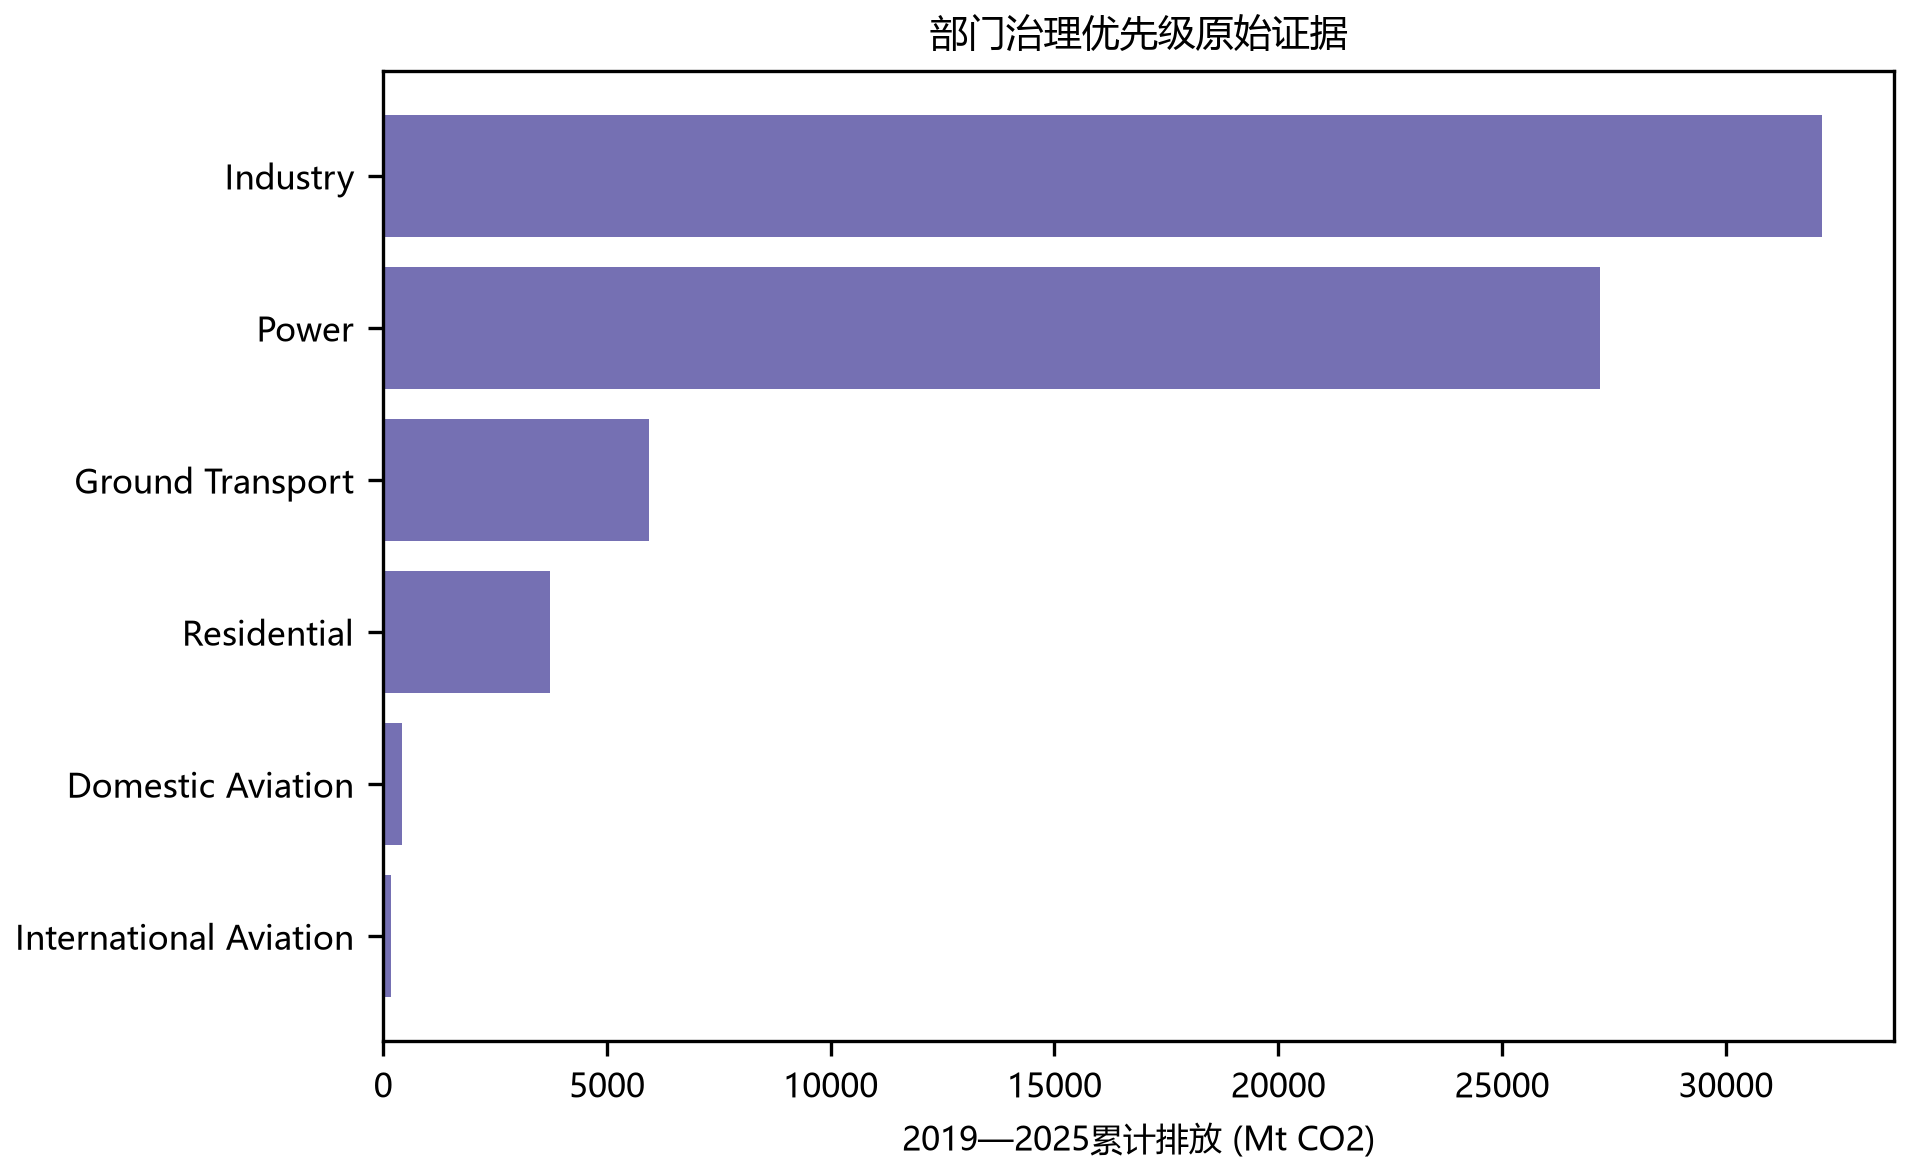
\includegraphics[width=0.86\textwidth]{figures/raw_q4_sector_share.png}
\caption{2019--2025年全国分部门累计排放及治理优先级（单位：Mt和\%）}
\label{fig:q4-raw}
\end{figure}
\vspace{-0.4\baselineskip}
\nopagebreak[4]
图\ref{fig:q4-raw}显示，工业和电力部门累计排放份额分别为46.20\%与39.08\%，两部门合计占全国累计排放的85.28\%，构成了减排的首要阵地。其余部门份额相对分散，治理优先级明显低于工业与电力。

\begin{figure}[H]
\centering
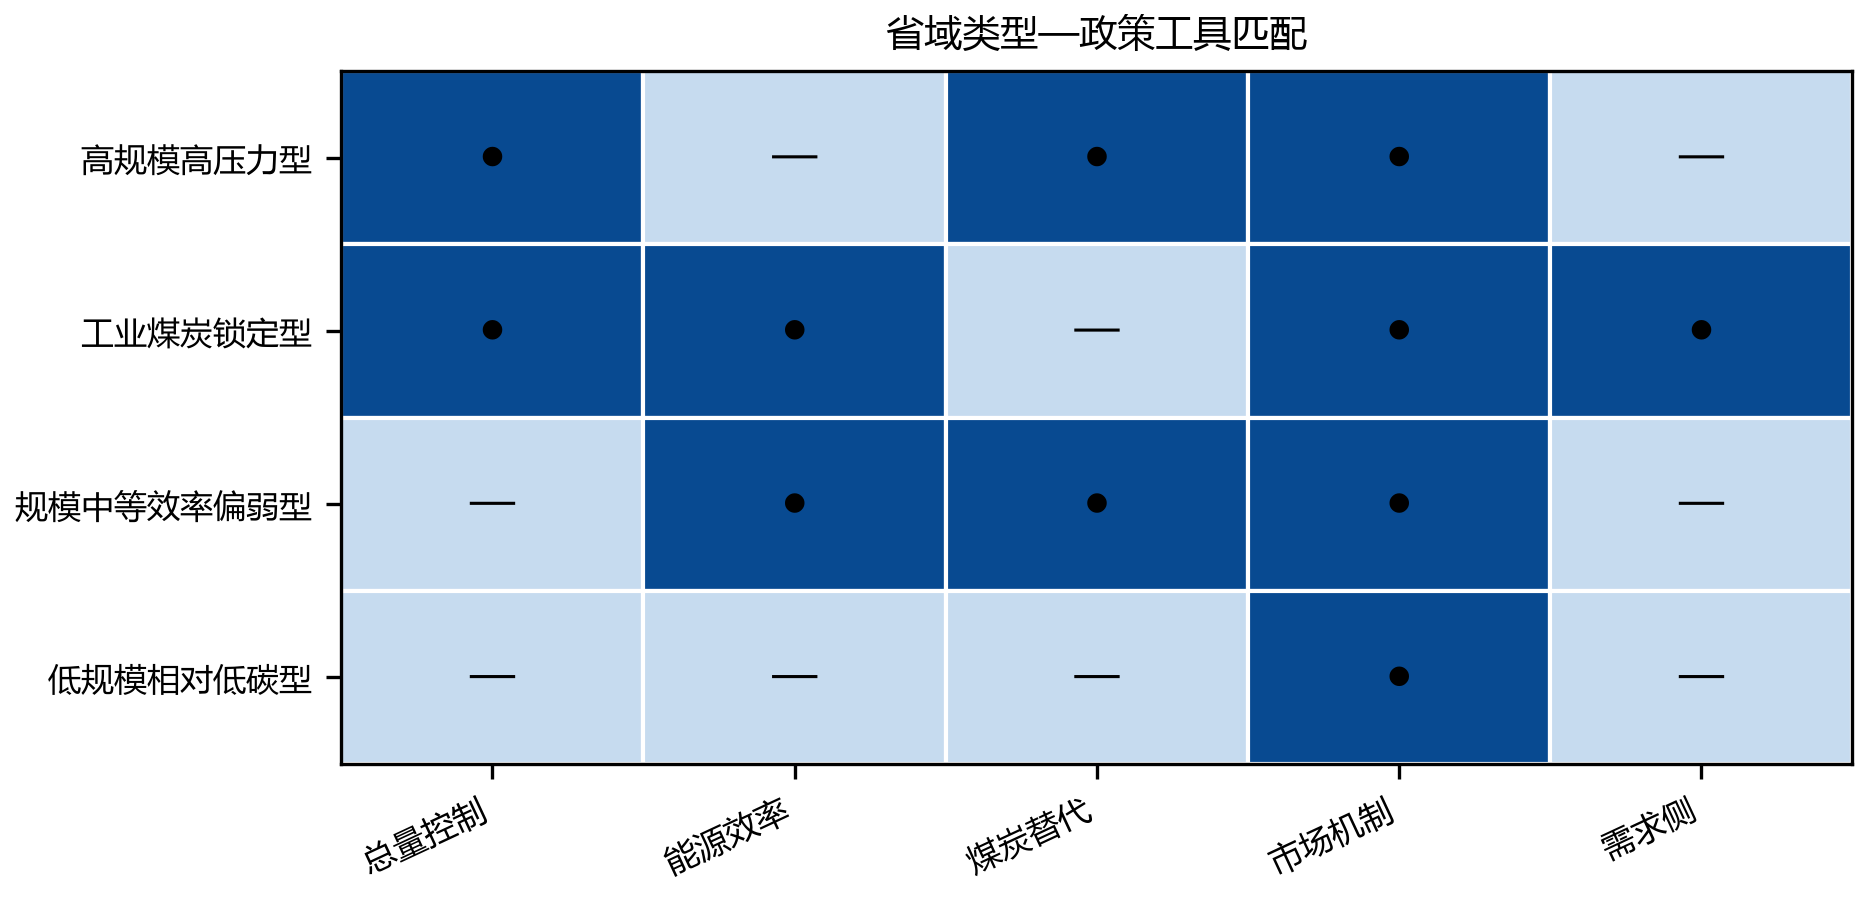
\includegraphics[width=0.90\textwidth]{figures/process_q4_policy_matrix.png}
\caption{按省级规则计算的类别政策工具覆盖率（单位：\%）}
\label{fig:q4-process}
\end{figure}
\vspace{-0.4\baselineskip}
\nopagebreak[4]
图\ref{fig:q4-process}显示，高规模高压力型在总量控制、能效改造和煤炭替代三类工具上的覆盖率明显高于其他类别，政策工具与类别画像高度匹配。

\begin{table}[H]
\centering
\caption{按省级规则计算的类别政策工具覆盖率}
\label{tab:q4-policy}
\zihao{5}
\resizebox{\textwidth}{!}{%
\begin{tabular}{lrrrrrr}
\toprule
类别 & 省份数 & 总量控制/(\%) & 能效改造/(\%) & 煤炭替代/(\%) & 市场机制/(\%) & 需求侧治理/(\%)\\
\midrule
高规模高压力型 & 8 & 100.0 & 87.5 & 100.0 & 62.5 & 0.0\\
低规模相对低碳型 & 21 & 4.8 & 38.1 & 33.3 & 47.6 & 23.8\\
低规模相对低碳型（结构差异簇） & 1 & 0.0 & 0.0 & 0.0 & 0.0 & 0.0\\
\bottomrule
\end{tabular}}
\end{table}
\vspace{-0.4\baselineskip}
\nopagebreak[4]
表\ref{tab:q4-policy}显示，高规模高压力型的总量控制和煤炭替代覆盖率均达100\%，能效改造覆盖率为87.5\%，该类别省份几乎全部触发刚性治理工具；低规模相对低碳型则更多依赖市场机制与需求侧工具，工具组合呈明显的差异化特征。

\begin{table}[H]
\centering
\caption{三情景阶段末排放强度指数与能源结构指标}
\label{tab:q4-phase}
\zihao{5}
\resizebox{\textwidth}{!}{%
\begin{tabular}{llrrrr}
\toprule
情景 & 阶段末 & 强度指数(2025=100) & 强度降幅/(\%) & 煤炭占比/(\%) & 清洁能源比重/(\%)\\
\midrule
基准 & 2030 & 84.44 & 15.56 & 49.4 & 32.6\\
基准 & 2035 & 72.61 & 27.39 & 46.4 & 35.6\\
基准 & 2045 & 55.70 & 44.30 & 40.4 & 41.6\\
低碳 & 2030 & 83.55 & 16.45 & 47.4 & 34.6\\
低碳 & 2035 & 71.24 & 28.76 & 42.4 & 39.6\\
低碳 & 2045 & 53.98 & 46.02 & 32.4 & 49.6\\
强化低碳 & 2030 & 83.27 & 16.73 & 45.4 & 36.6\\
强化低碳 & 2035 & 70.97 & 29.03 & 38.4 & 43.6\\
强化低碳 & 2045 & 54.34 & 45.66 & 24.4 & 57.6\\
\bottomrule
\end{tabular}}
\end{table}
\vspace{-0.4\baselineskip}
\nopagebreak[4]
表\ref{tab:q4-phase}显示，三情景强度指数均随阶段稳步下降，至2045年降至53.98至55.70之间，较2025年降幅达44.30\%至46.02\%，各阶段的强度目标可量化、可检查，为年度滚动监测提供了基准。

\begin{figure}[H]
\centering
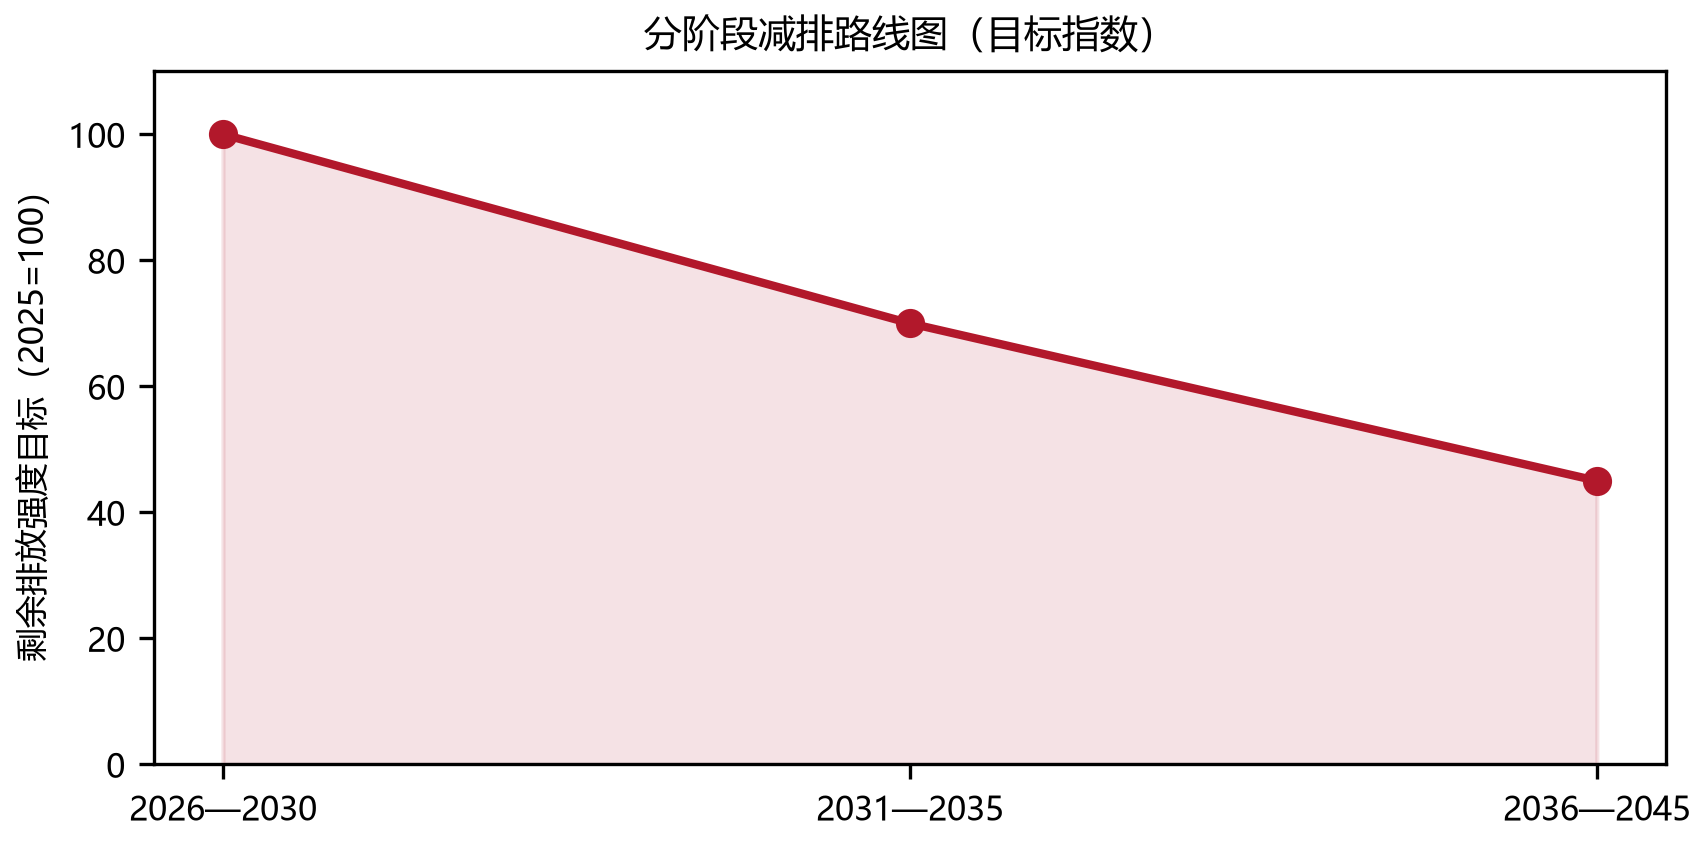
\includegraphics[width=0.86\textwidth]{figures/result_q4_roadmap.png}
\caption{由情景预测结果计算的三情景阶段末强度指数}
\label{fig:q4-result}
\end{figure}
\vspace{-0.4\baselineskip}
\nopagebreak[4]
图\ref{fig:q4-result}汇总了三情景的阶段末强度指数，强化低碳情景在2035年前下降最快，低碳情景的2045年强度指数最低，说明转型力度越大的路径越早显现降碳成效，也提示分阶段考核应随情景差异设置不同的目标值。

\subsubsection{本文结论}

结合前述空间聚类、宏观驱动及多情景推演结果，系统提出面向我国碳达峰与碳中和目标的政策建议书：
\begin{enumerate}[label=\textbf{(\arabic*)}]
\item \textbf{分区域靶向施策：} 对8个高规模高压力型省份全面实施刚性碳预算控制、煤炭替代（覆盖率$100.0\%$）与能效改造（$87.5\%$）；对21个低规模相对低碳型省份依托市场机制（$47.6\%$）推进碳市场履约与设备节能改造；对北京发挥低碳技术与碳资产管理策源功能。
\item \textbf{分部门深度脱碳：} 聚焦累计排放占比达$85.28\%$的工业（$46.20\%$）与电力（$39.08\%$）两大核心阵地，实施工业工艺绿色再造与新型电力系统建设。
\item \textbf{三阶段稳步推进：} 制定“2026--2030年达峰筑基（强度指数降至$83.27\sim84.44$）、2031--2035年平台攻坚（强度指数降至$70.97\sim72.61$）、2036--2045年深度脱碳（强度指数降至$53.98\sim55.70$）”三步走路线。
\item \textbf{全流程动态监测：} 建立涵盖总量、强度、煤炭占比与重点部门排放的五维监测看板，实施年度滚动复盘与预警纠偏。
\end{enumerate}

\section{模型评价与推广}

\subsection{模型优点}
四个问题采用“区域识别--驱动分析--情景预测--政策建议”的顺序：横截面模型用于说明地区之间的差异，时间序列模型用于讨论全国排放与驱动变量的共同变化，情景模型用于比较给定路径下的长期变化，政策映射则把分析结果转化为分层措施。各环节的统计对象和时间尺度不同，因此需要结合各自的适用范围理解结果。
\begin{enumerate}[label=(\arabic*)]
\item 先进行\texttt{Total}口径核验并区分全国时间序列和省级横截面，避免把不同来源、不同层级的数据重复计量。
\item 对空间差异同时报告Moran检验、轮廓系数和分类解释，并以轮廓系数最大规则确定$k=3$，使分类决策可由结果表复核。
\item STIRPAT-ridge将能源结构方向约束纳入估计，并以扩展窗口MAE与时间趋势基线比较，避免仅报告样本内拟合误差。
\item 政策建议由省域类别、部门结构、情景差异和监测指标逐层映射，能够支持年度滚动复盘。
\end{enumerate}

\subsection{模型的缺点}
\begin{enumerate}[label=(\arabic*)]
\item 全国驱动模型只有6个年度观测，参数不确定性较大；模型系数只能做结构性解释，不能作为因果效应或精确长期点预测。
\item 省级样本不含西藏，海南采用桥接空间关系；全局Moran检验不能替代基于真实经济联系、能源流或电网拓扑的空间网络分析。
\item 外生GDP和能源结构路径是情景假设而非官方规划，经验残差带也不是正式置信区间；2045年边界最大值不能证明已经达峰。
\item 聚类只依赖五项静态指标，尽管$k=3$在候选范围内的轮廓系数最高，类别仍应理解为描述性画像。后续可增加更长时间序列、分省能源价格、技术进步、产业结构和跨区电力交换数据，构造面板STIRPAT、空间面板或状态空间模型。
\end{enumerate}

\subsection{模型的推广}
本文的分析框架可以推广到省级面板排放、行业排放或城市排放研究。若进一步获得跨省电力流、产业链联系、能源价格和技术改造成本等数据，可在现有指标体系上构建空间面板模型或多目标优化模型；同时保留“区域识别--驱动分析--情景预测--政策建议”的基本思路，实现更精细的碳排放治理分析。

\section*{AI 工具使用声明}
\addcontentsline{toc}{section}{AI 工具使用声明}
\noindent 本参赛队在竞赛过程中使用了 AI 工具，主要用于简要用途，如语言润色、数据读取和代码调试等，详细使用情况见支撑材料。

\begin{thebibliography}{99}
\raggedright
\addcontentsline{toc}{section}{参考文献}
\bibitem{moran} Moran, P. A. P. Notes on Continuous Stochastic Phenomena[J]. Biometrika, 1950, 37(1/2): 17--23. DOI: 10.1093/biomet/37.1-2.17.
\bibitem{ward} Ward, J. H. Hierarchical Grouping to Optimize an Objective Function[J]. Journal of the American Statistical Association, 1963, 58(301): 236--244. DOI: 10.1080/00401658.1963.10500845.
\bibitem{stats} 国家统计局. 《中国统计年鉴2023》, 表2-7、表3-9、表9-2. \url{https://www.stats.gov.cn/sj/ndsj/2023/}.
\bibitem{stirpat} York, R., Rosa, E. A., Dietz, T. Footprints on the Earth: The Environmental Consequences of Modernity[J]. American Sociological Review, 2003, 68(2): 279--300. DOI: 10.2307/1519769.
\bibitem{ridge} Hoerl, A. E., Kennard, R. W. Ridge Regression: Biased Estimation for Nonorthogonal Problems[J]. Technometrics, 1970, 12(1): 55--67. DOI: 10.1080/00401706.1970.10488634.

\end{thebibliography}

\newpage
\appendix
\renewcommand{\thesection}{附录 \Alph{section}}
\renewcommand{\thesubsection}{\Alph{section}.\arabic{subsection}}
\renewcommand{\thesubsubsection}{\Alph{section}.\arabic{subsection}.\arabic{subsubsection}}
\titleformat{\section}{\centering\heiti\zihao{-3}\bfseries}{\thesection}{1em}{}

\section{支撑文件列表}

本论文的支撑材料共包含~4~个求解程序、14~个结果数据表与~1~份~AI~工具使用说明，文件清单与用途如下表所示。

\begin{longtable}{>{\raggedright\arraybackslash}p{6.5cm}>{\raggedright\arraybackslash}p{7.8cm}}
\caption{支撑材料文件清单与说明}\label{tab:support}\\
\toprule
文件 & 说明 \\
\midrule
\endfirsthead
\toprule
文件 & 说明 \\
\midrule
\endhead
\bottomrule
\endlastfoot
\texttt{problem\_1.py} & 问题一求解代码 \\
\texttt{problem\_2.py} & 问题二求解代码 \\
\texttt{problem\_3.py} & 问题三求解代码 \\
\texttt{problem\_4.py} & 问题四求解代码 \\
\texttt{q1\_省级指标与分类.csv} & 30~省份五维指标与聚类分类结果 \\
\texttt{q1\_Moran检验.csv} & 全局~Moran's~I~及置 换检验~$p$~值 \\
\texttt{q1\_分组差异检验.csv} & 各类别间~Kruskal--Wallis~差异检验 \\
\texttt{q1\_PCA.csv} & 主成分方差解释率 \\
\texttt{q1\_聚类稳定性.csv} & 不同~$k$~下聚类稳定性 \\
\texttt{q1\_聚类决策.csv} & 轮廓系数随~$k$~变化与最优~$k$~选择 \\
\texttt{q2\_驱动因素系数.csv} & STIRPAT-ridge~标准化系数及相对权重 \\
\texttt{q2\_回测.csv} & 扩展窗口外推~MAE/RMSE~回测误差 \\
\texttt{q3\_2026-2045\_三情景预测.csv} & 2026--2045~三情景逐年排放总量与强度 \\
\texttt{q3\_情景约束检查.csv} & 能源结构约束满足性检查 \\
\texttt{q4\_省级政策映射.csv} & 30~省份政策工具映射 \\
\texttt{q4\_类别政策覆盖率.csv} & 各聚类类别政策覆盖率 \\
\texttt{q4\_阶段情景指标.csv} & 三阶段强度指数与减排目标 \\
\texttt{q4\_部门优先级.csv} & 部门累计排放占比与脱碳优先级 \\
\texttt{AI工具使用详情.pdf} & AI~辅助工具使用说明与声明 \\
\end{longtable}

\section{相关代码}


\subsection{问题一：空间格局与聚类（problem\_1.py）}
\lstinputlisting[language=Python, caption={问题一求解代码 problem\_1.py}, label={lst:q1}]{code/problem_1.py}

\subsection{问题二：驱动因素识别（problem\_2.py）}
\lstinputlisting[language=Python, caption={问题二求解代码 problem\_2.py}, label={lst:q2}]{code/problem_2.py}

\subsection{问题三：情景预测（problem\_3.py）}
\lstinputlisting[language=Python, caption={问题三求解代码 problem\_3.py}, label={lst:q3}]{code/problem_3.py}

\subsection{问题四：政策映射（problem\_4.py）}
\lstinputlisting[language=Python, caption={问题四求解代码 problem\_4.py}, label={lst:q4}]{code/problem_4.py}

\end{document}






